\graphicspath{{chapt_dutch/}{intro/}{chapt2/}{chapt3/}{chapt4/}{chapt5/}{chapt6/}{chapt7/}{chapt8/}}

% Header
\renewcommand\evenpagerightmark{{\scshape\small Appendix C}}
\renewcommand\oddpageleftmark{{\scshape\small Data MC comparison}}

\renewcommand{\bibname}{References}

\hyphenation{}

\chapter[Data MC comparison]%
{Data MC comparison}\label{app4}
Figures below show distributions of a number of basic observables after the full event selection.
All corrections are applied and an overall good description of data is observed, with the notable exception of variables related to pileup, Primary Vertices (PV).
This mismodelling is a known result of the dynamic tracker inefficiency and its mitigation in reconstruction algorithms, and it is absorbed in the calibration of physics objects and in corresponding scale factors. The figures also show large statistical fluctuations in the multijet background.
This is a direct result of the small effective integrated luminosities of some of the simulated samples.
This problem has been addressed in a data-driven description of the multijet background constructed in Section~\ref{Sec:DataDrivenQCD}.
\begin{figure}
  \centering
  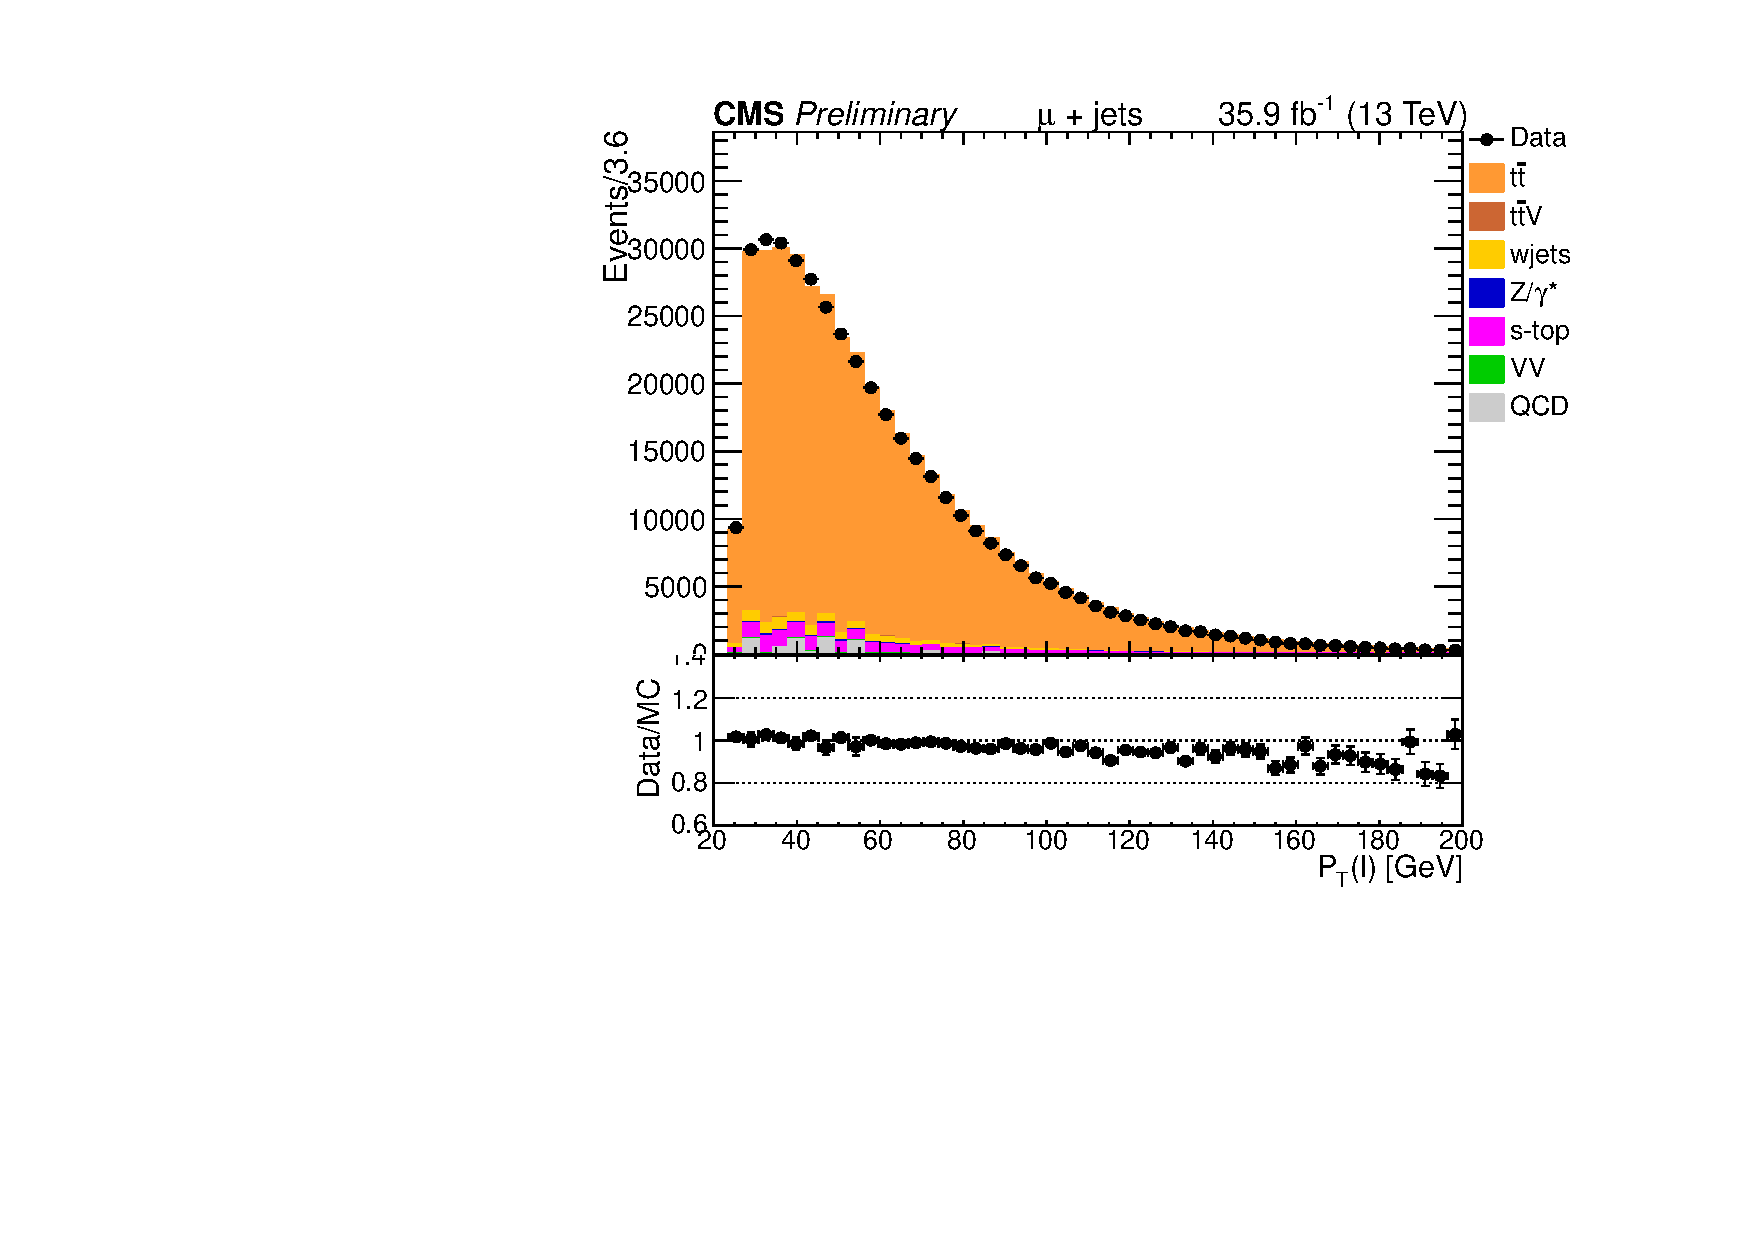
\includegraphics[width=0.45\textwidth]{fig/app4/muon/Pt_lep.pdf}
  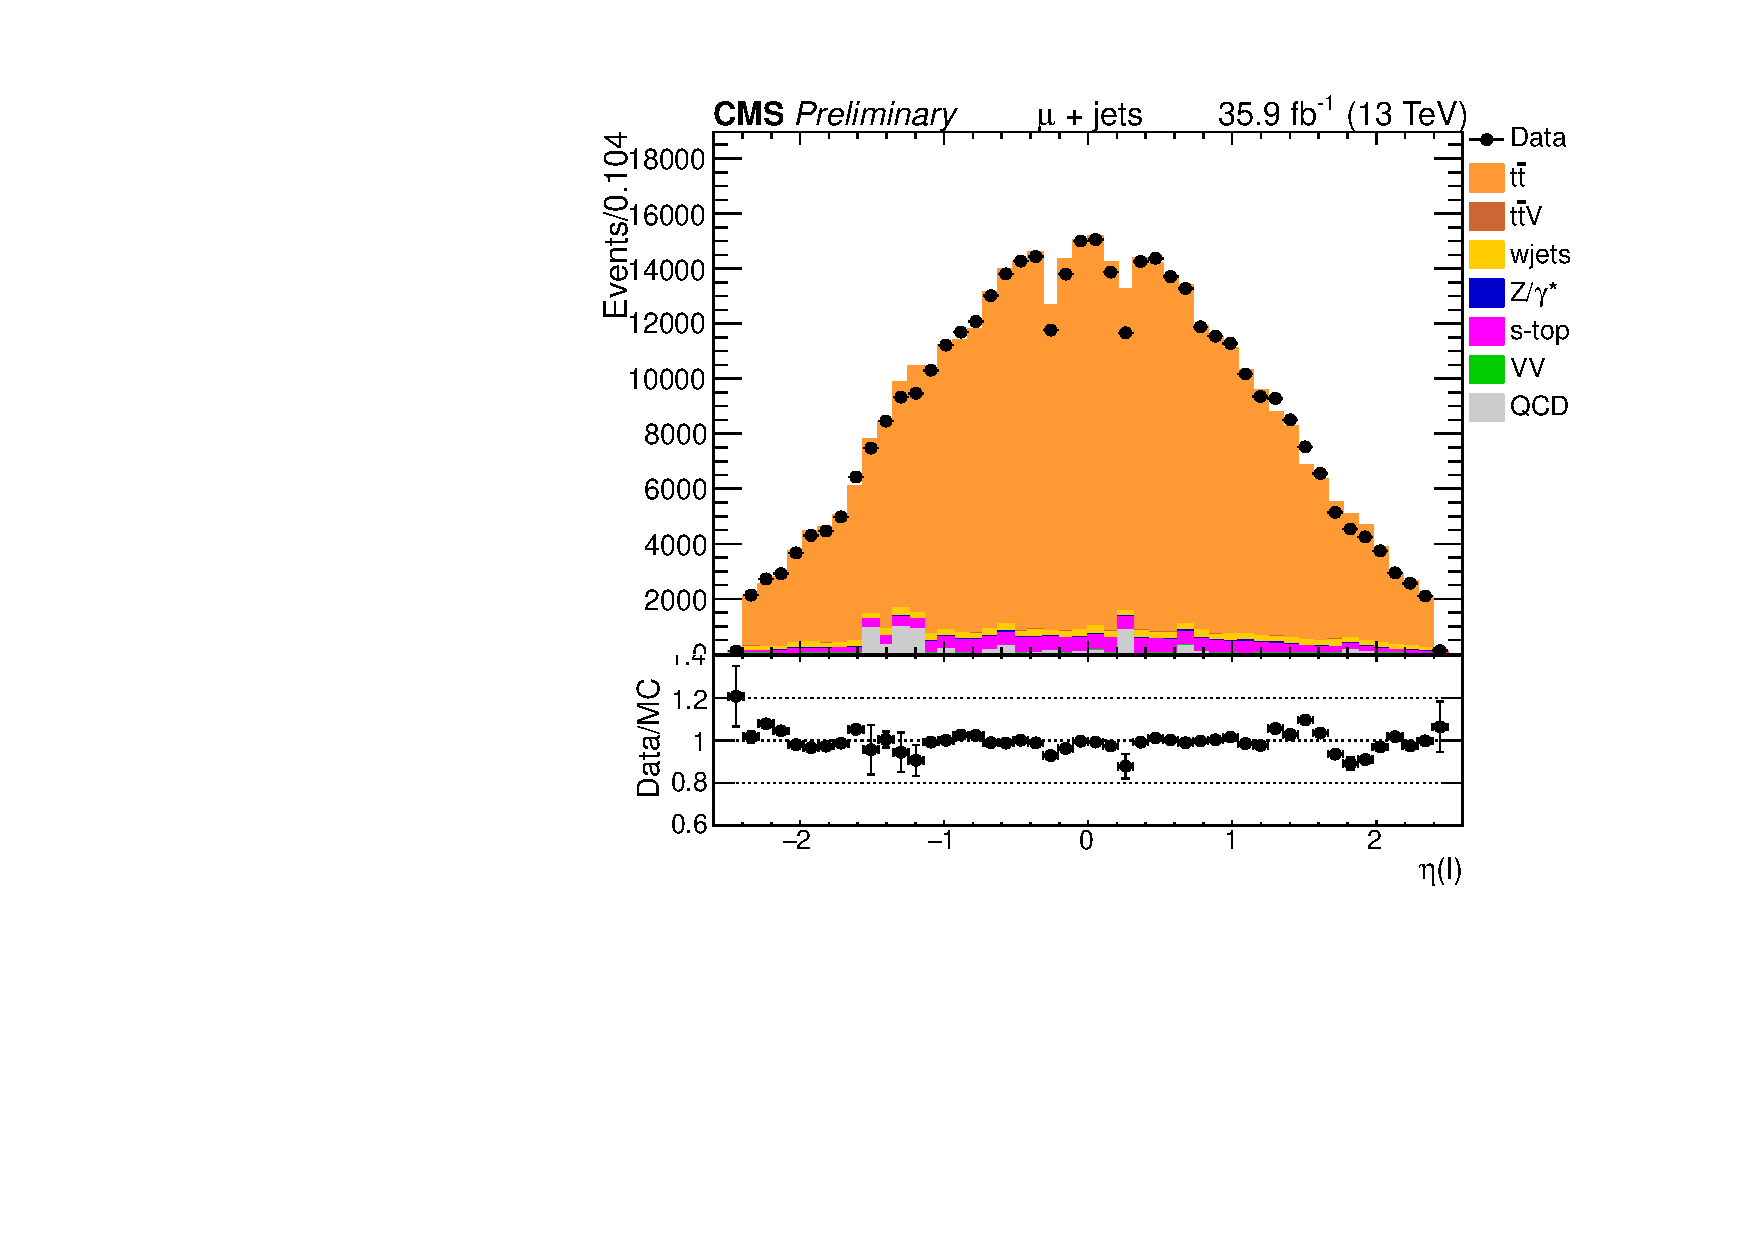
\includegraphics[width=0.45\textwidth]{fig/app4/muon/Eta_lep.pdf} \\
  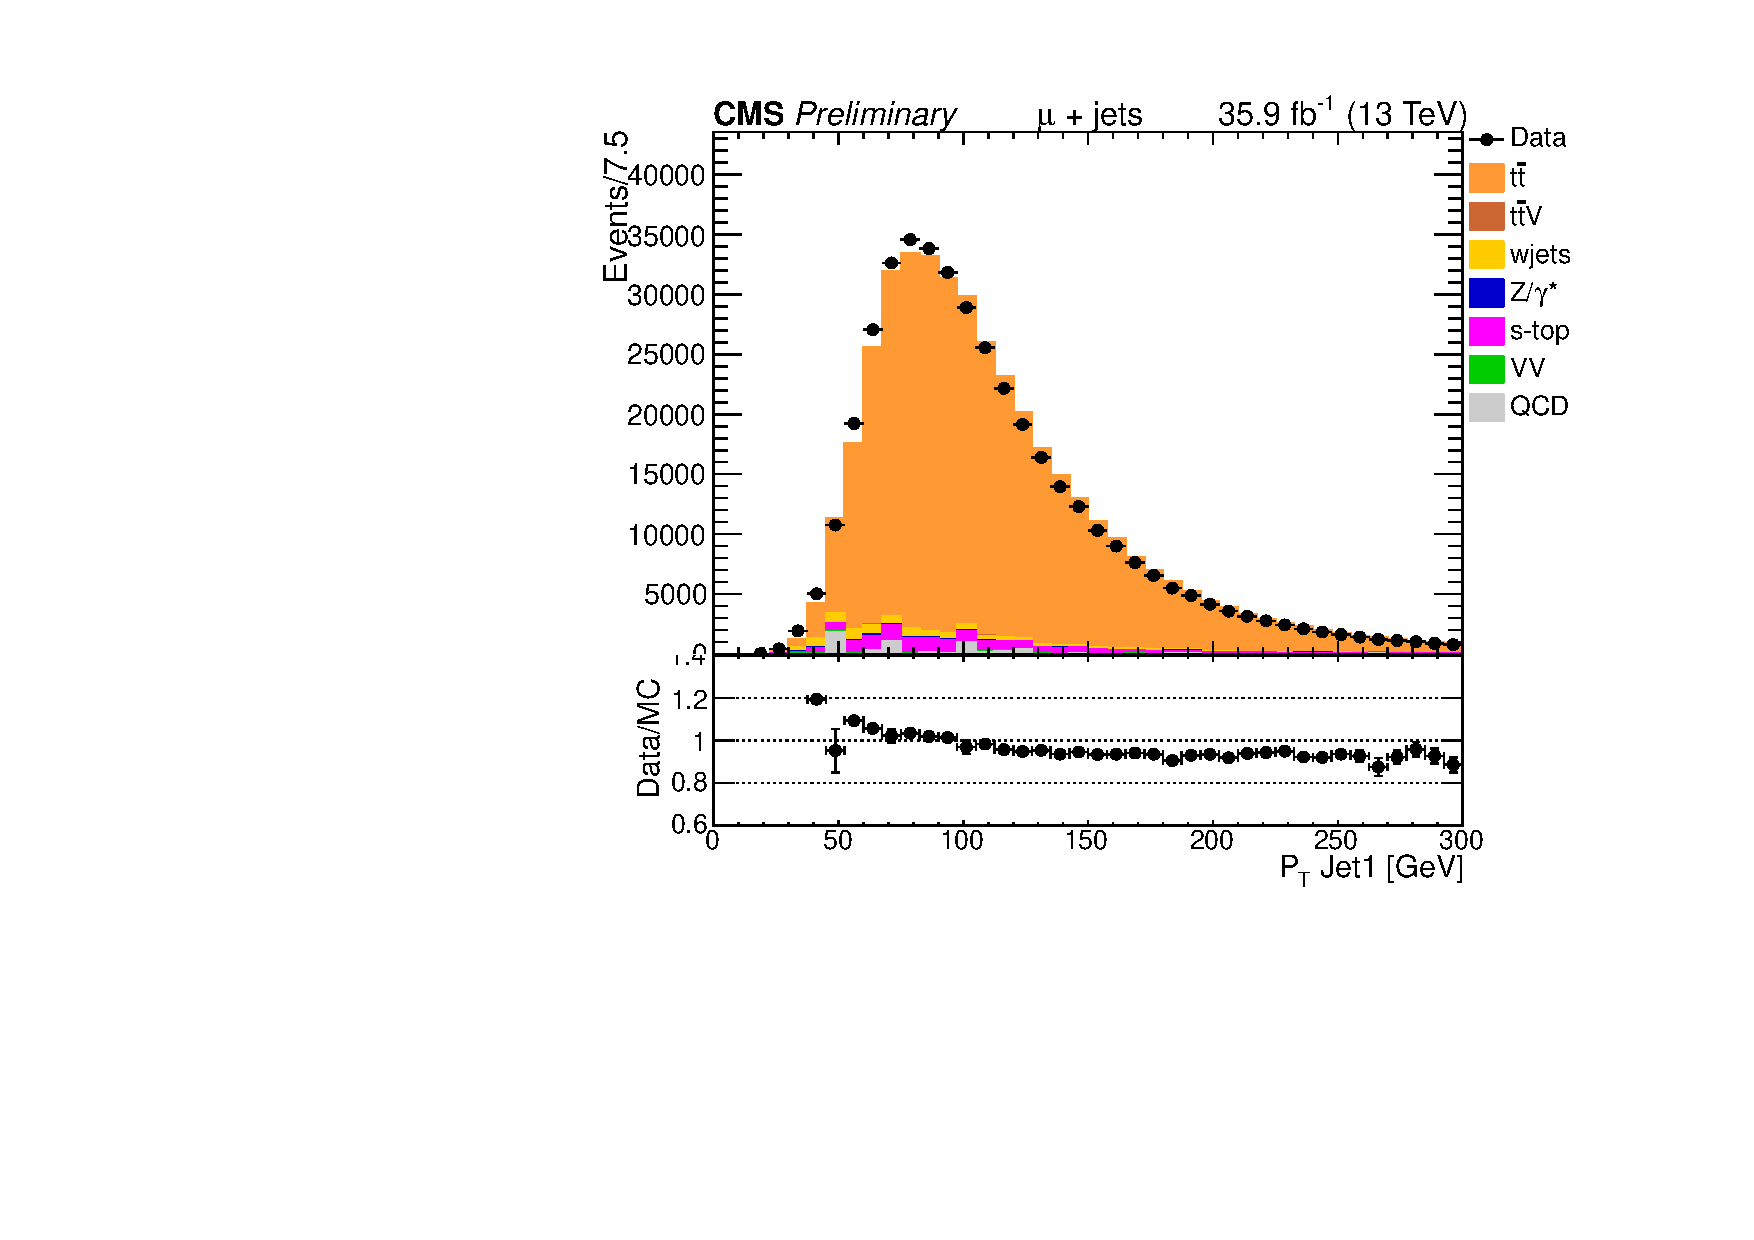
\includegraphics[width=0.45\textwidth]{fig/app4/muon/PtJet1.pdf}
  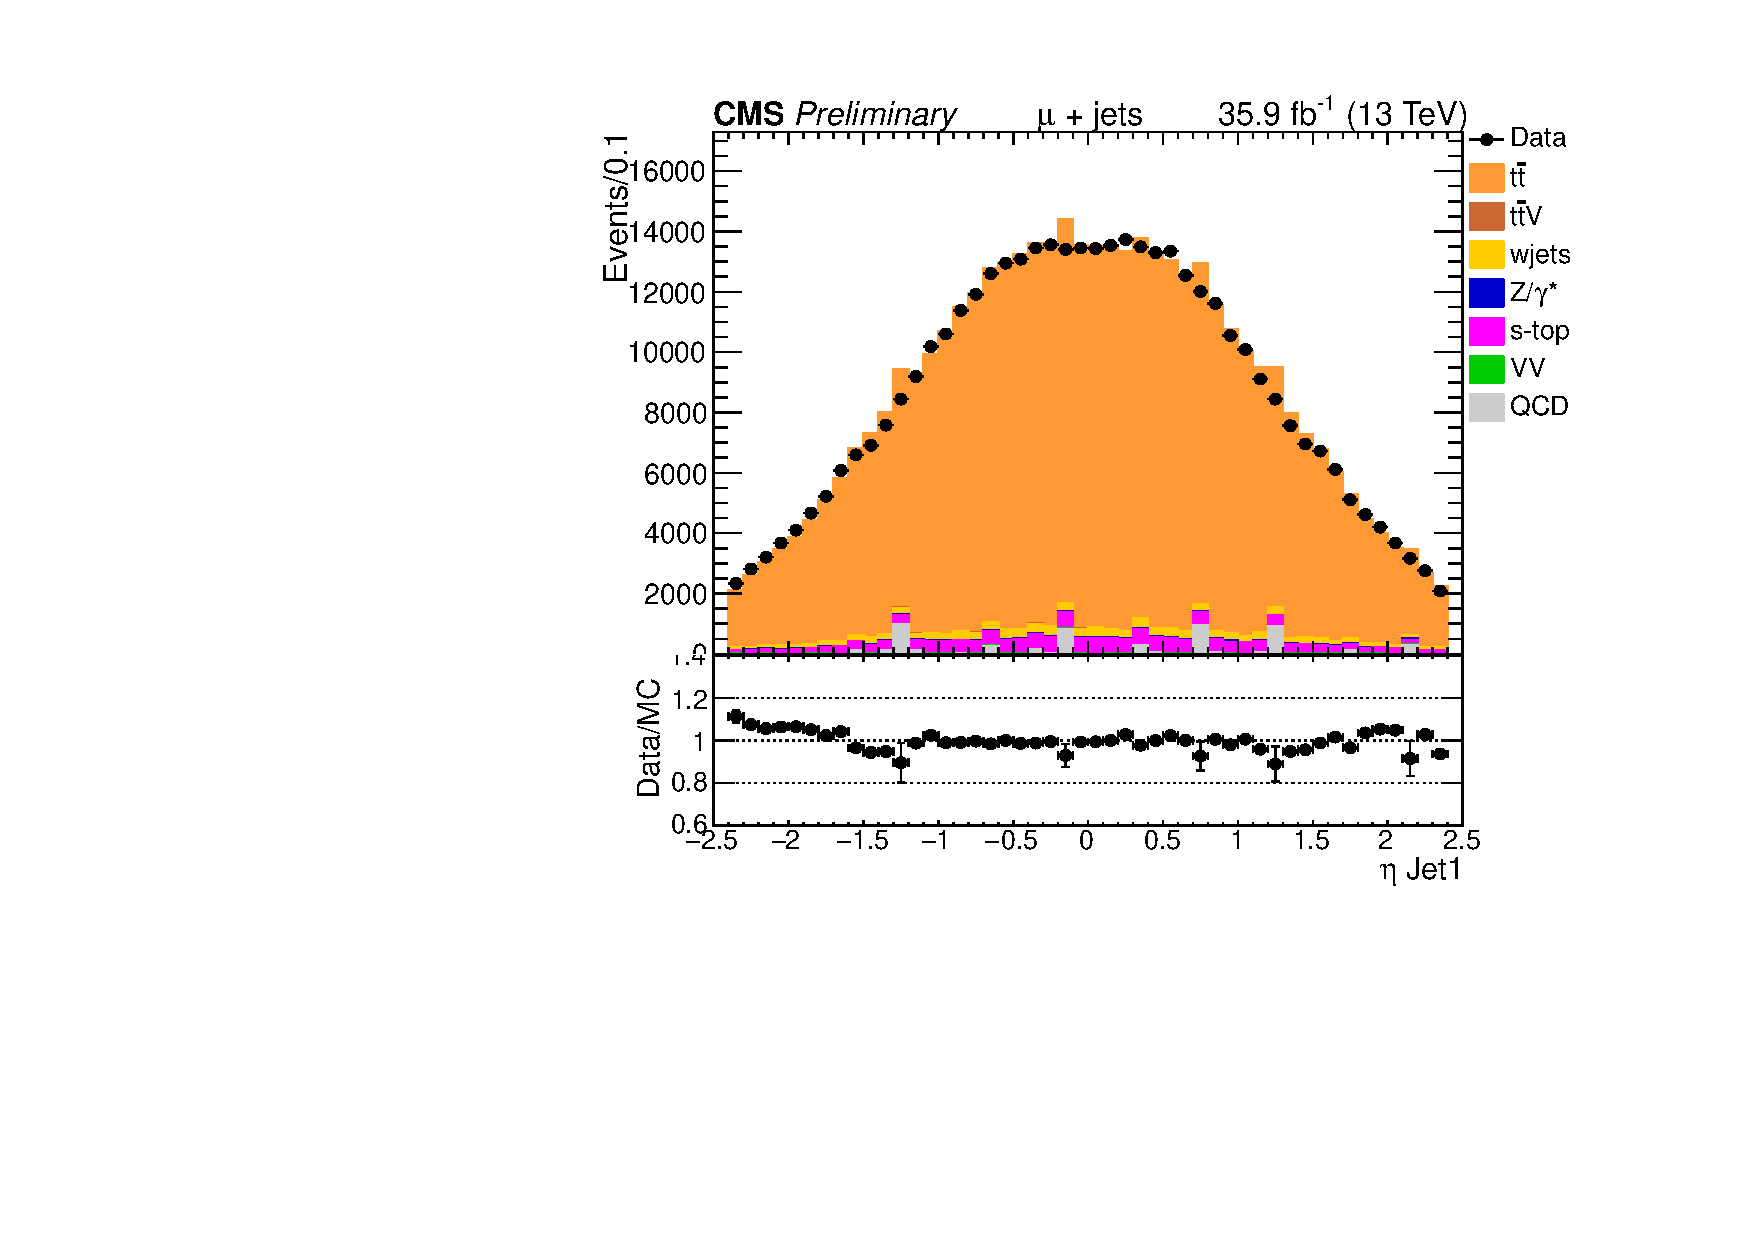
\includegraphics[width=0.45\textwidth]{fig/app4/muon/EtaJet1.pdf}
  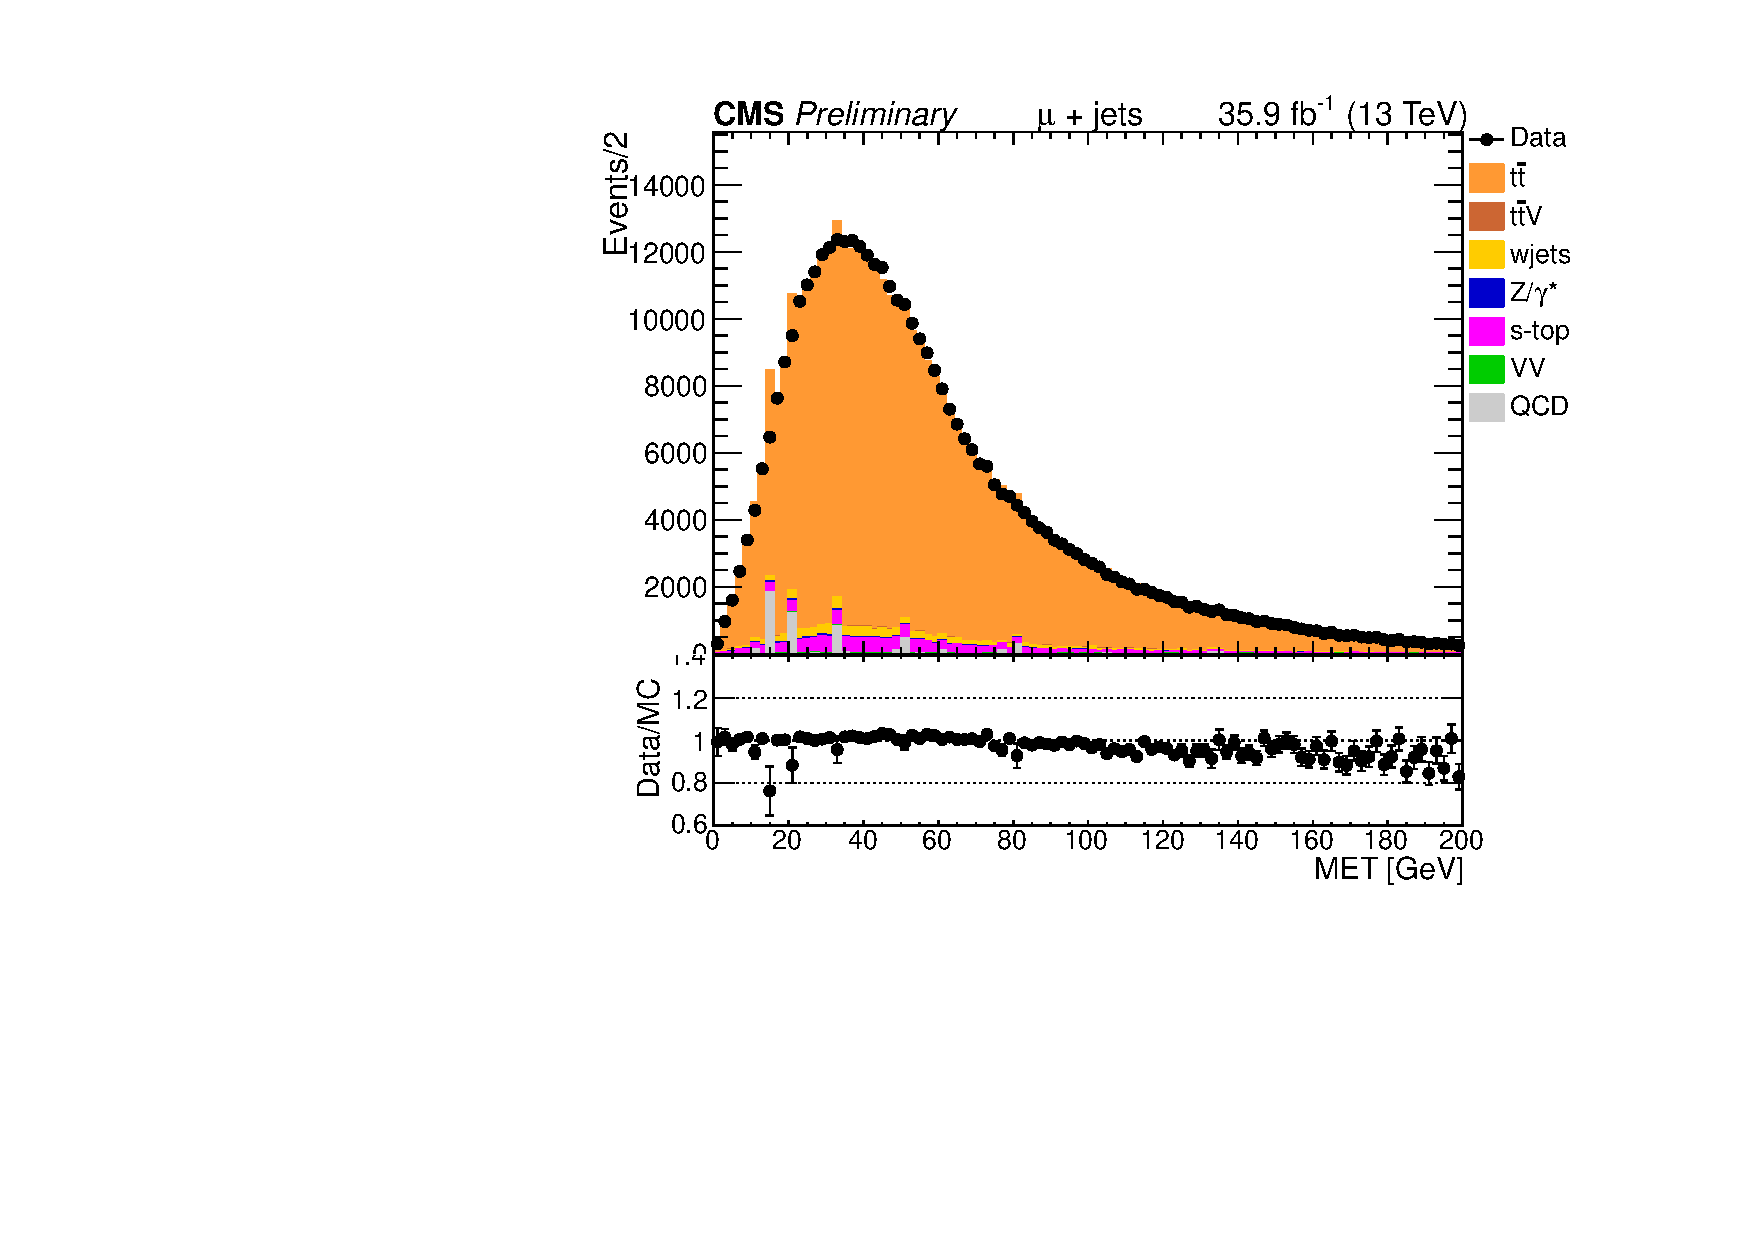
\includegraphics[width=0.45\textwidth]{fig/app4/muon/MET_E.pdf}
  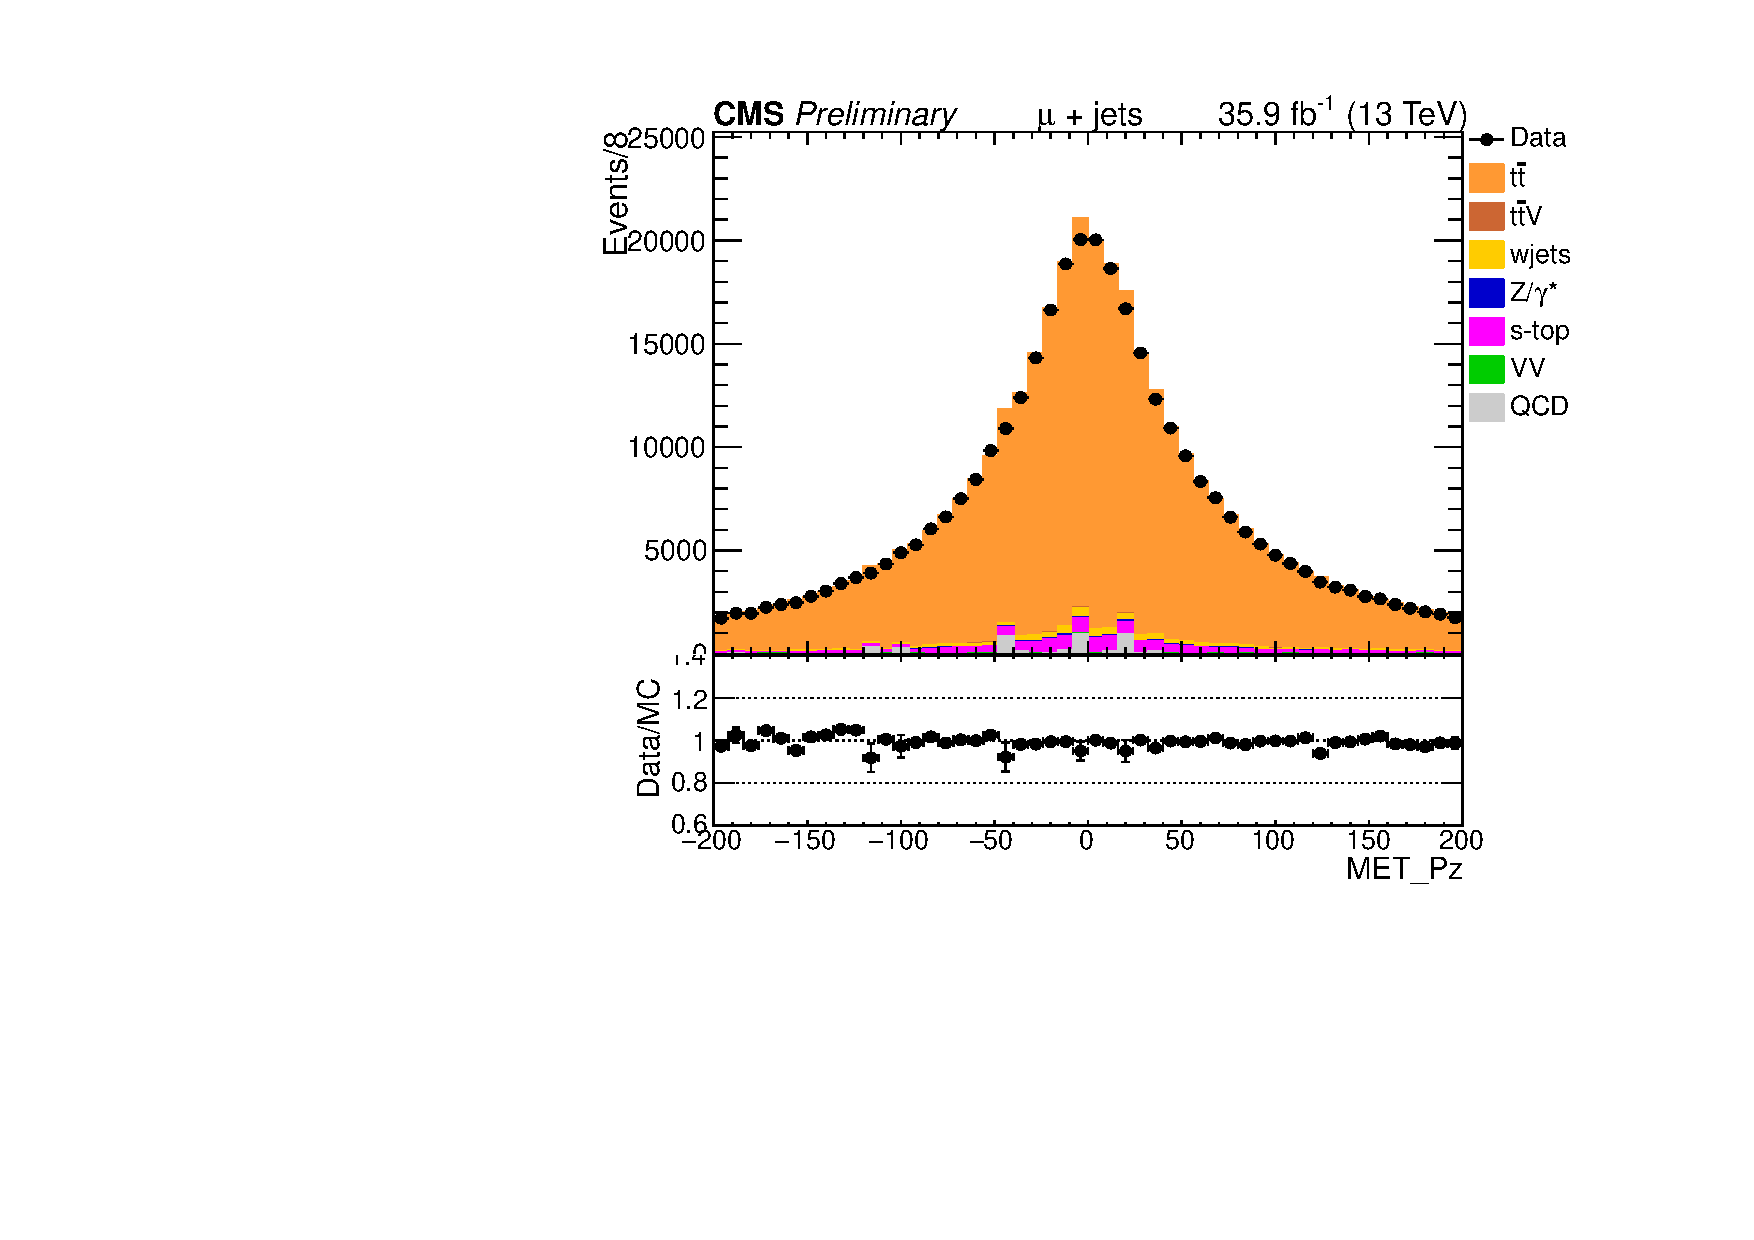
\includegraphics[width=0.45\textwidth]{fig/app4/muon/MET_Pz.pdf}
  \caption{Basic variables distributions in muon channel, from left to right, transverse momentum, $p_{T}$, and pseudorapidity, $\eta$, of muon, $p_{T}$ and $\eta$ of leading $p_{T}$ jets, missing transverse energy, $p_{T}^{\text{miss}}$, and the corresponding reconstructed $p_{Z}$ of $p_{T}^{\text{miss}}$.}
  \label{Fig:DataMCMuon1}
  \end{figure}

\begin{figure}
  \centering
  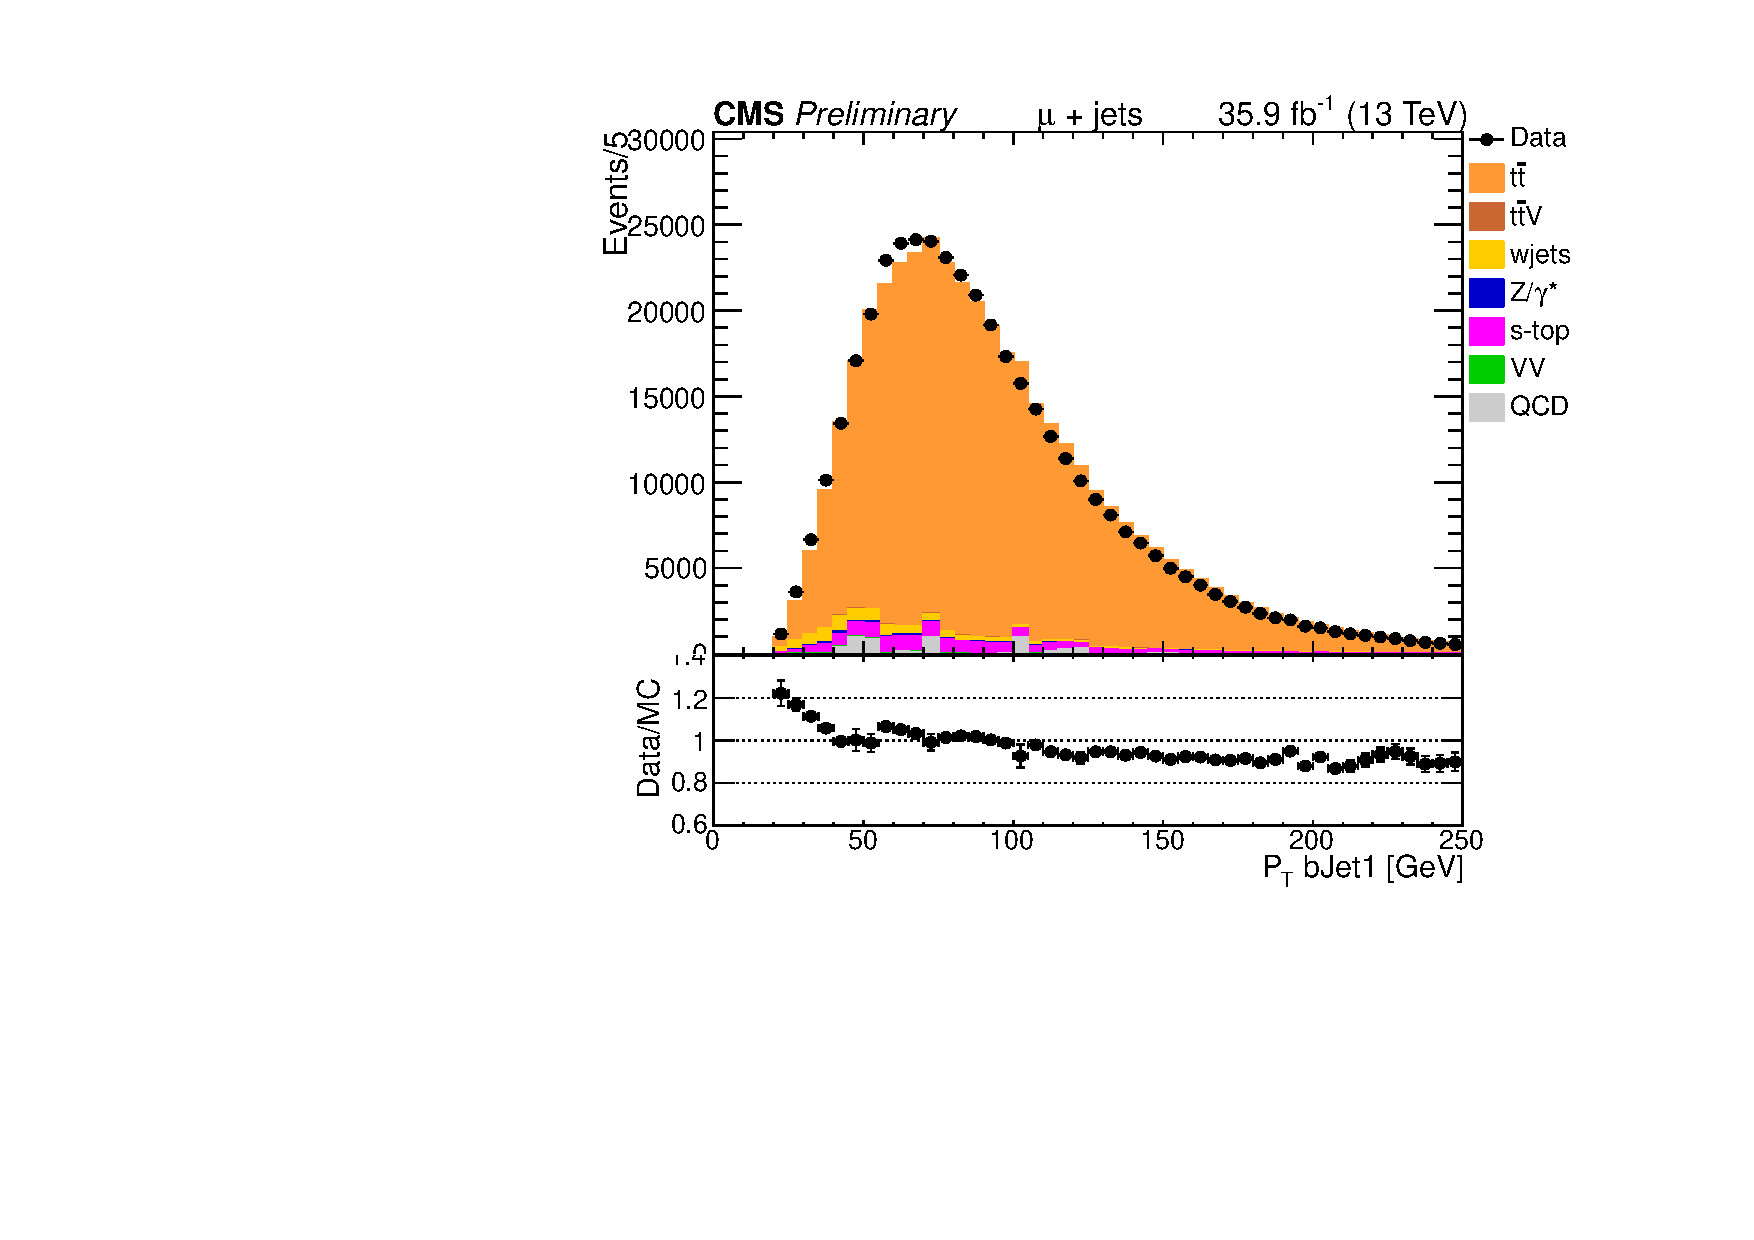
\includegraphics[width=0.45\textwidth]{fig/app4/muon/Pt_bJet1.pdf}
  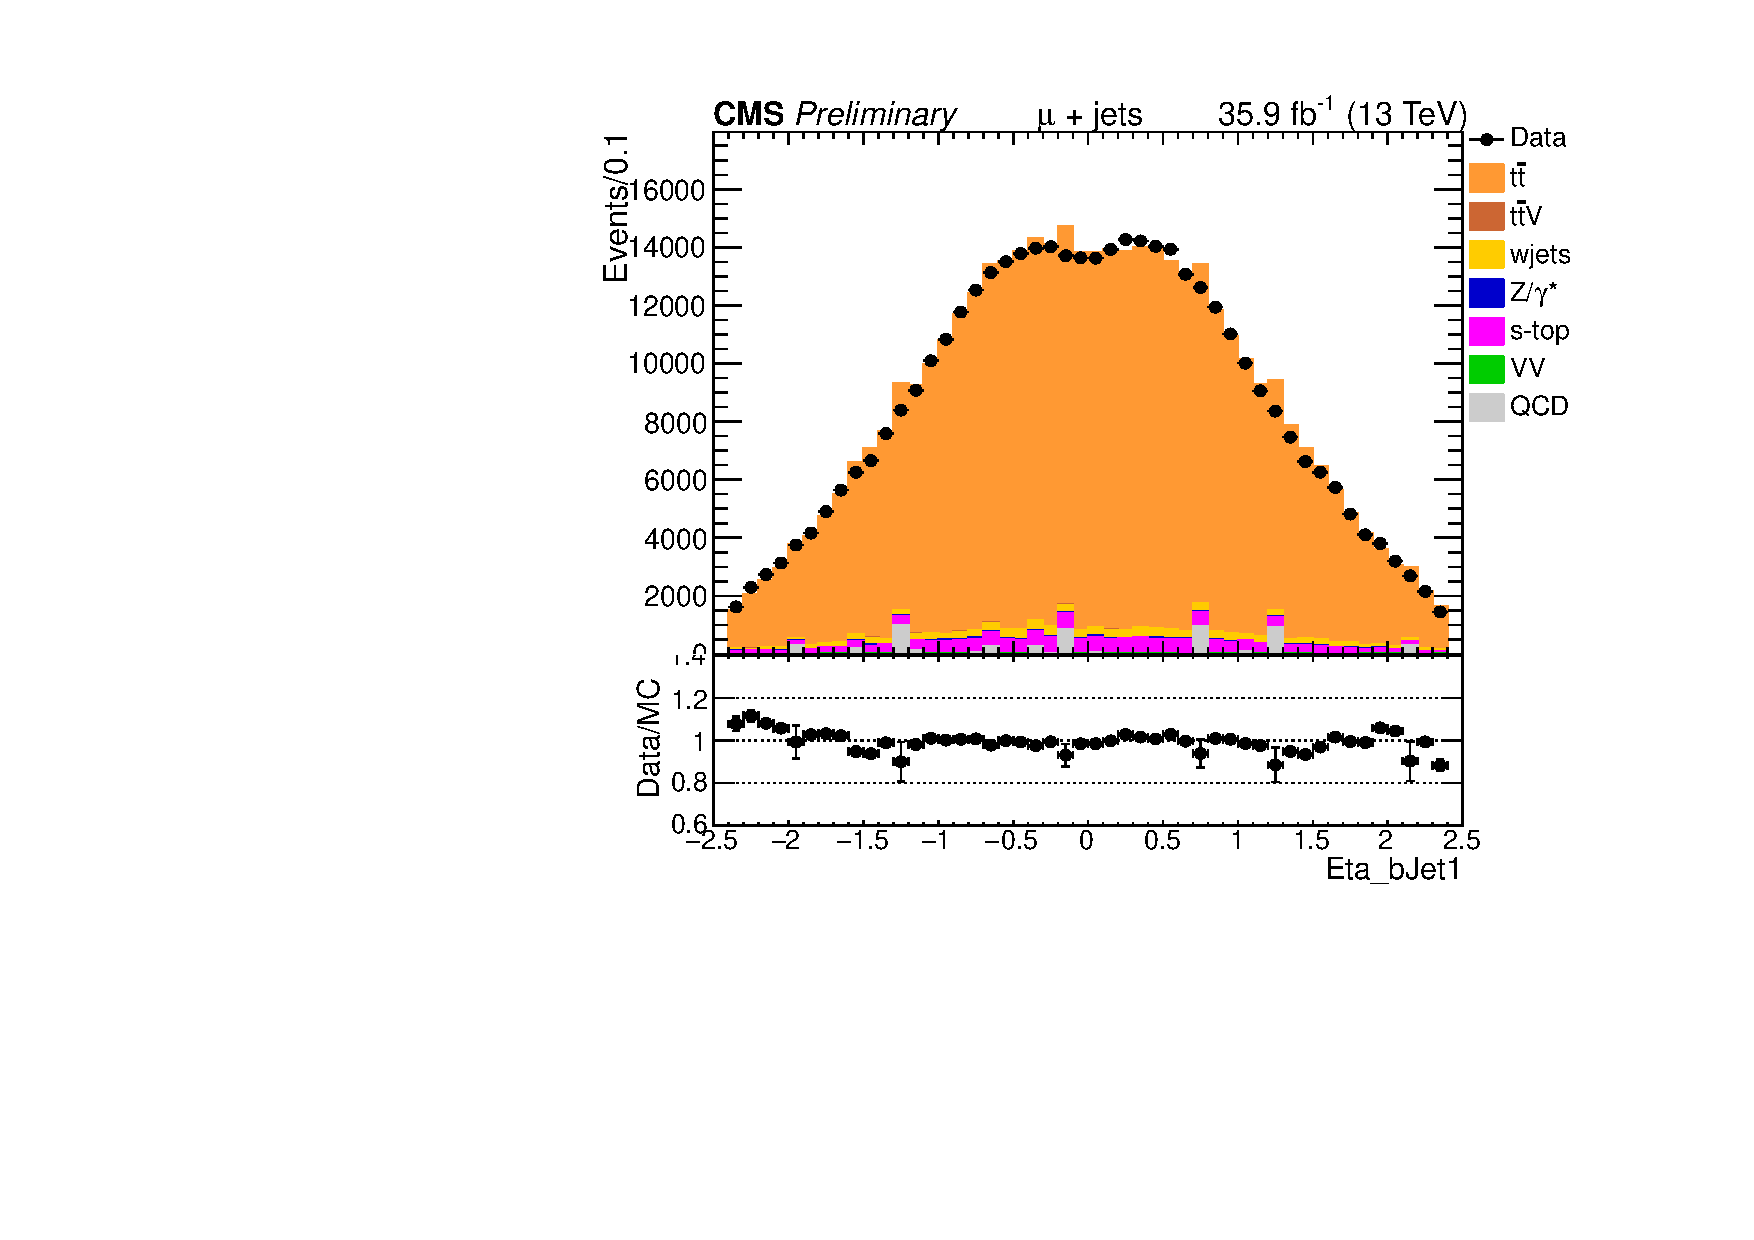
\includegraphics[width=0.45\textwidth]{fig/app4/muon/Eta_bJet1.pdf} \\
  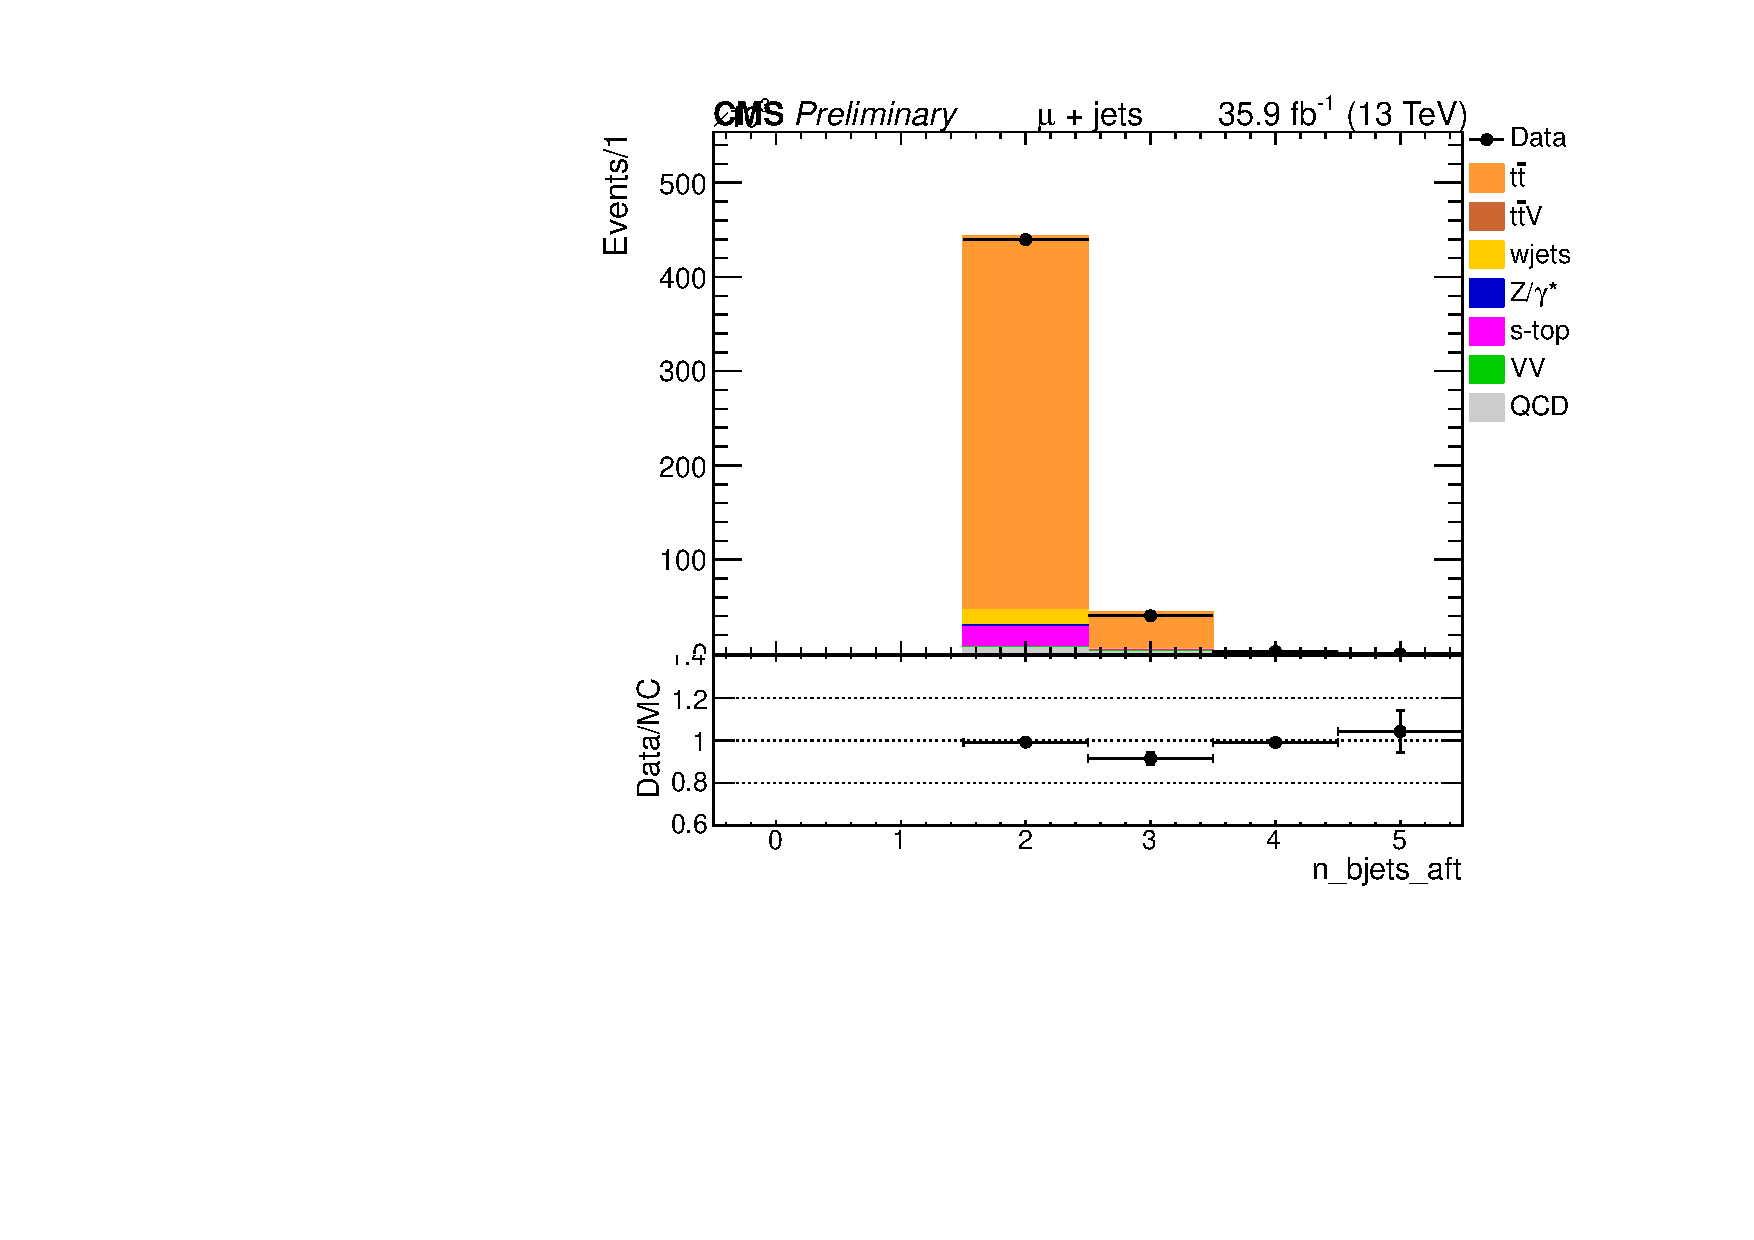
\includegraphics[width=0.45\textwidth]{fig/app4/muon/n_bJets_aft.pdf}
  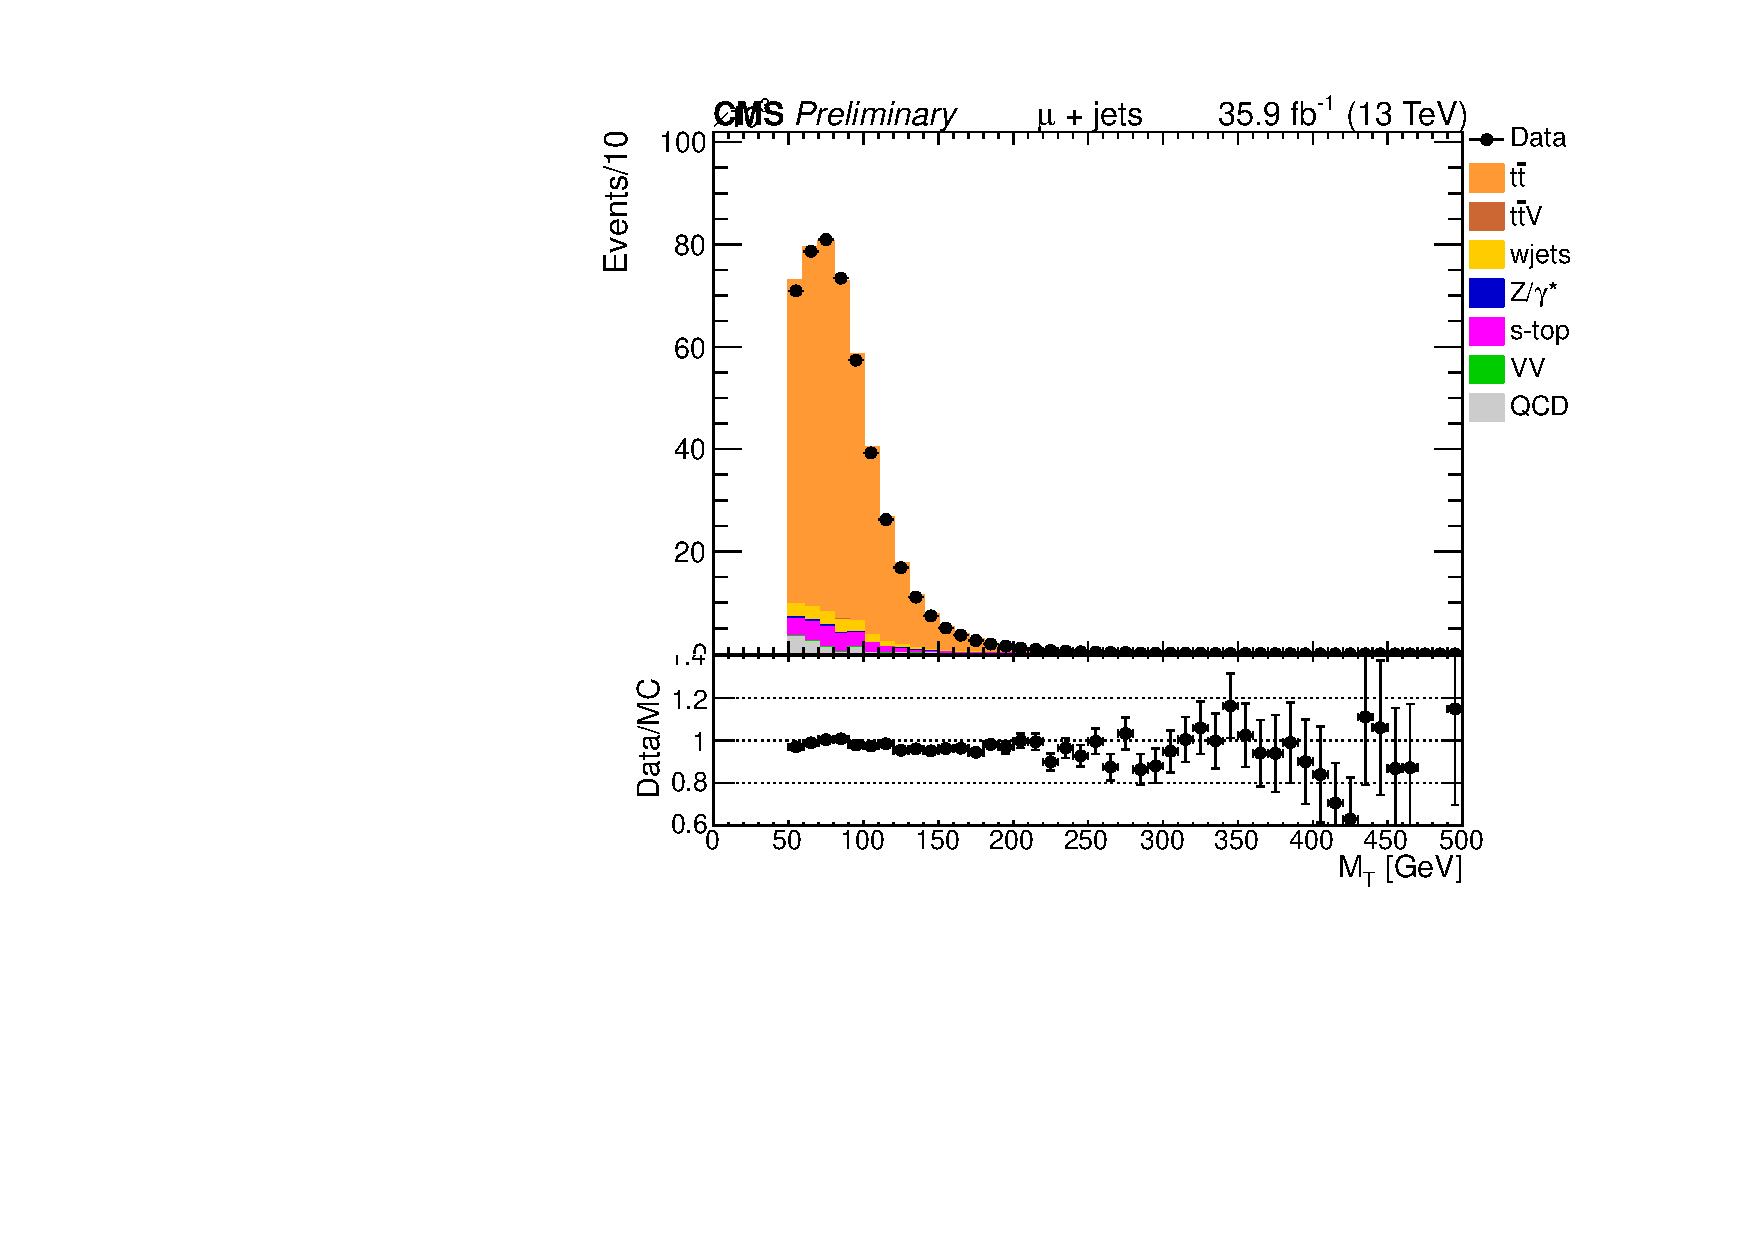
\includegraphics[width=0.45\textwidth]{fig/app4/muon/M_T_aft.pdf}
  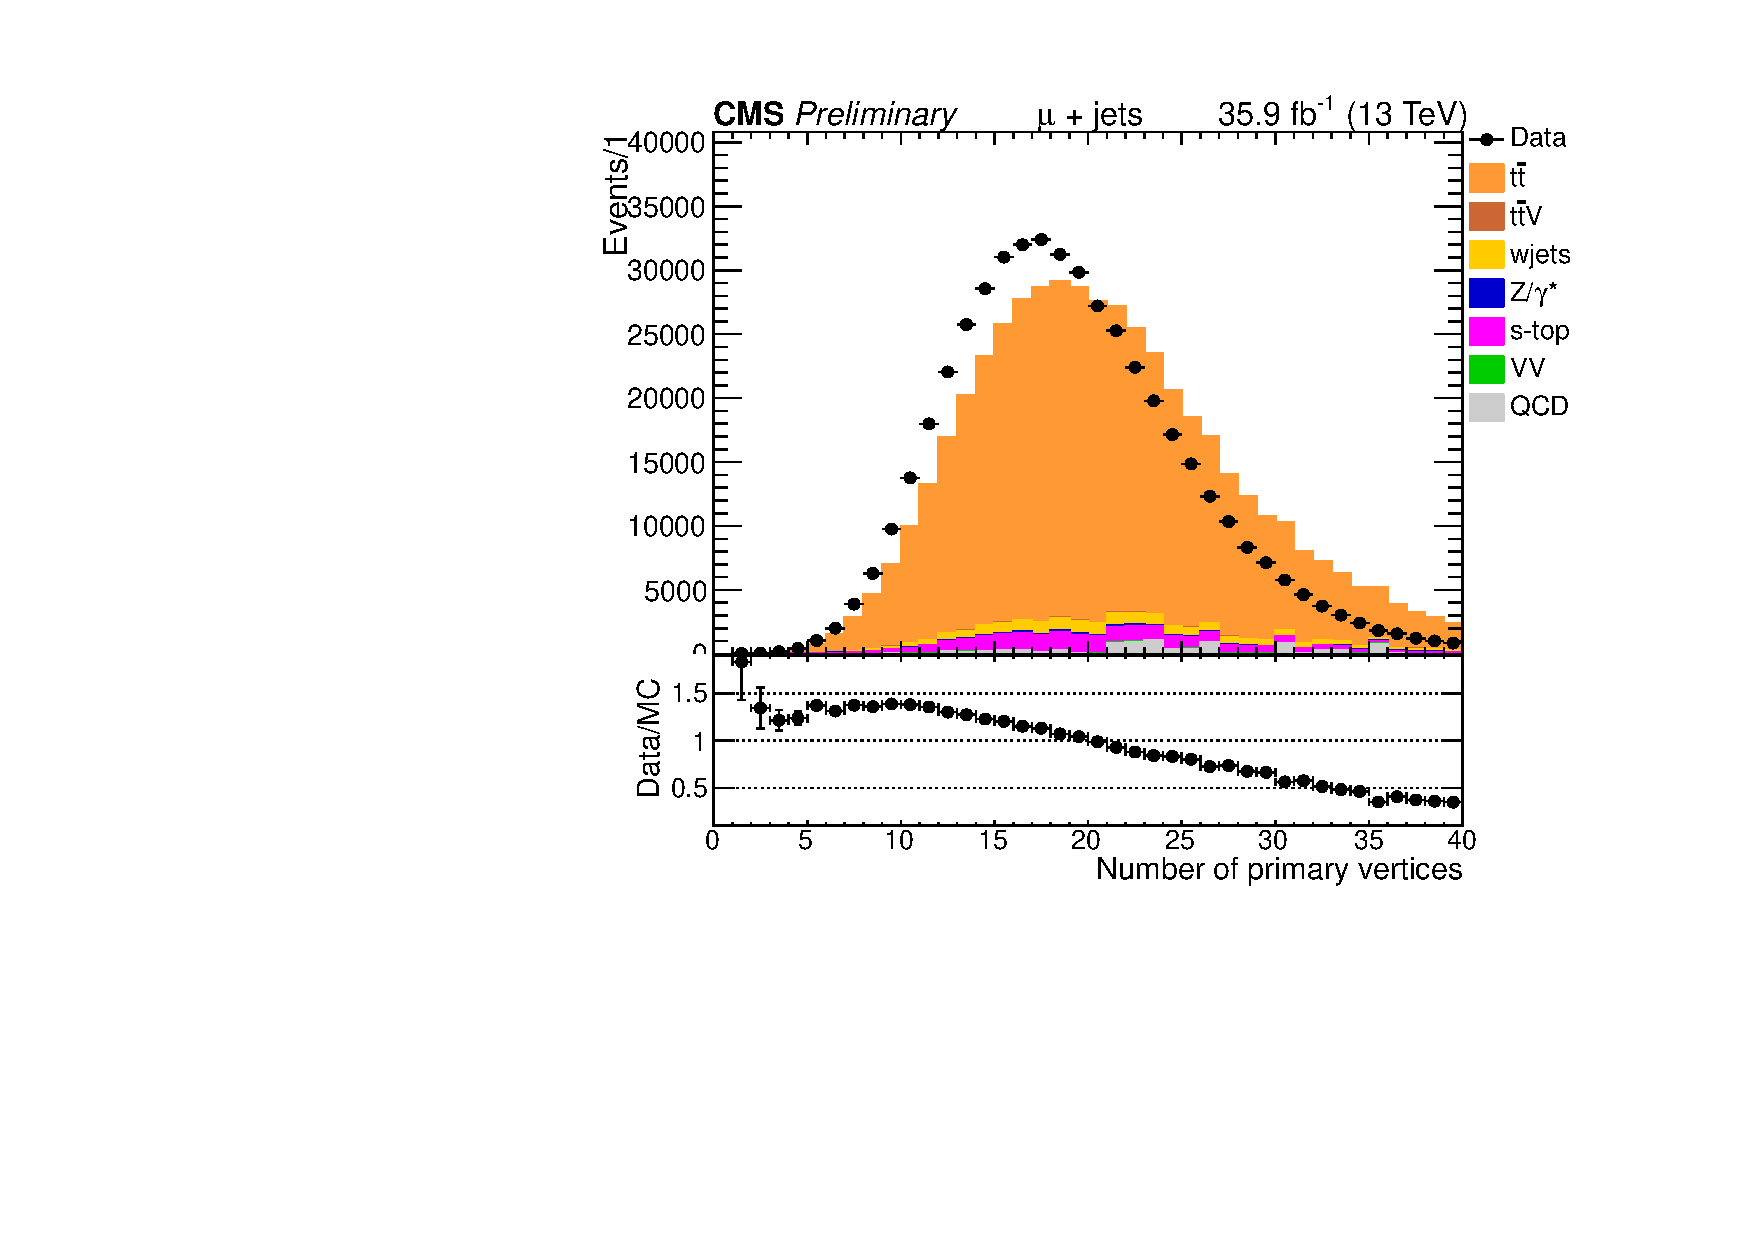
\includegraphics[width=0.45\textwidth]{fig/app4/muon/EvtInfo_NumVtx.pdf}
  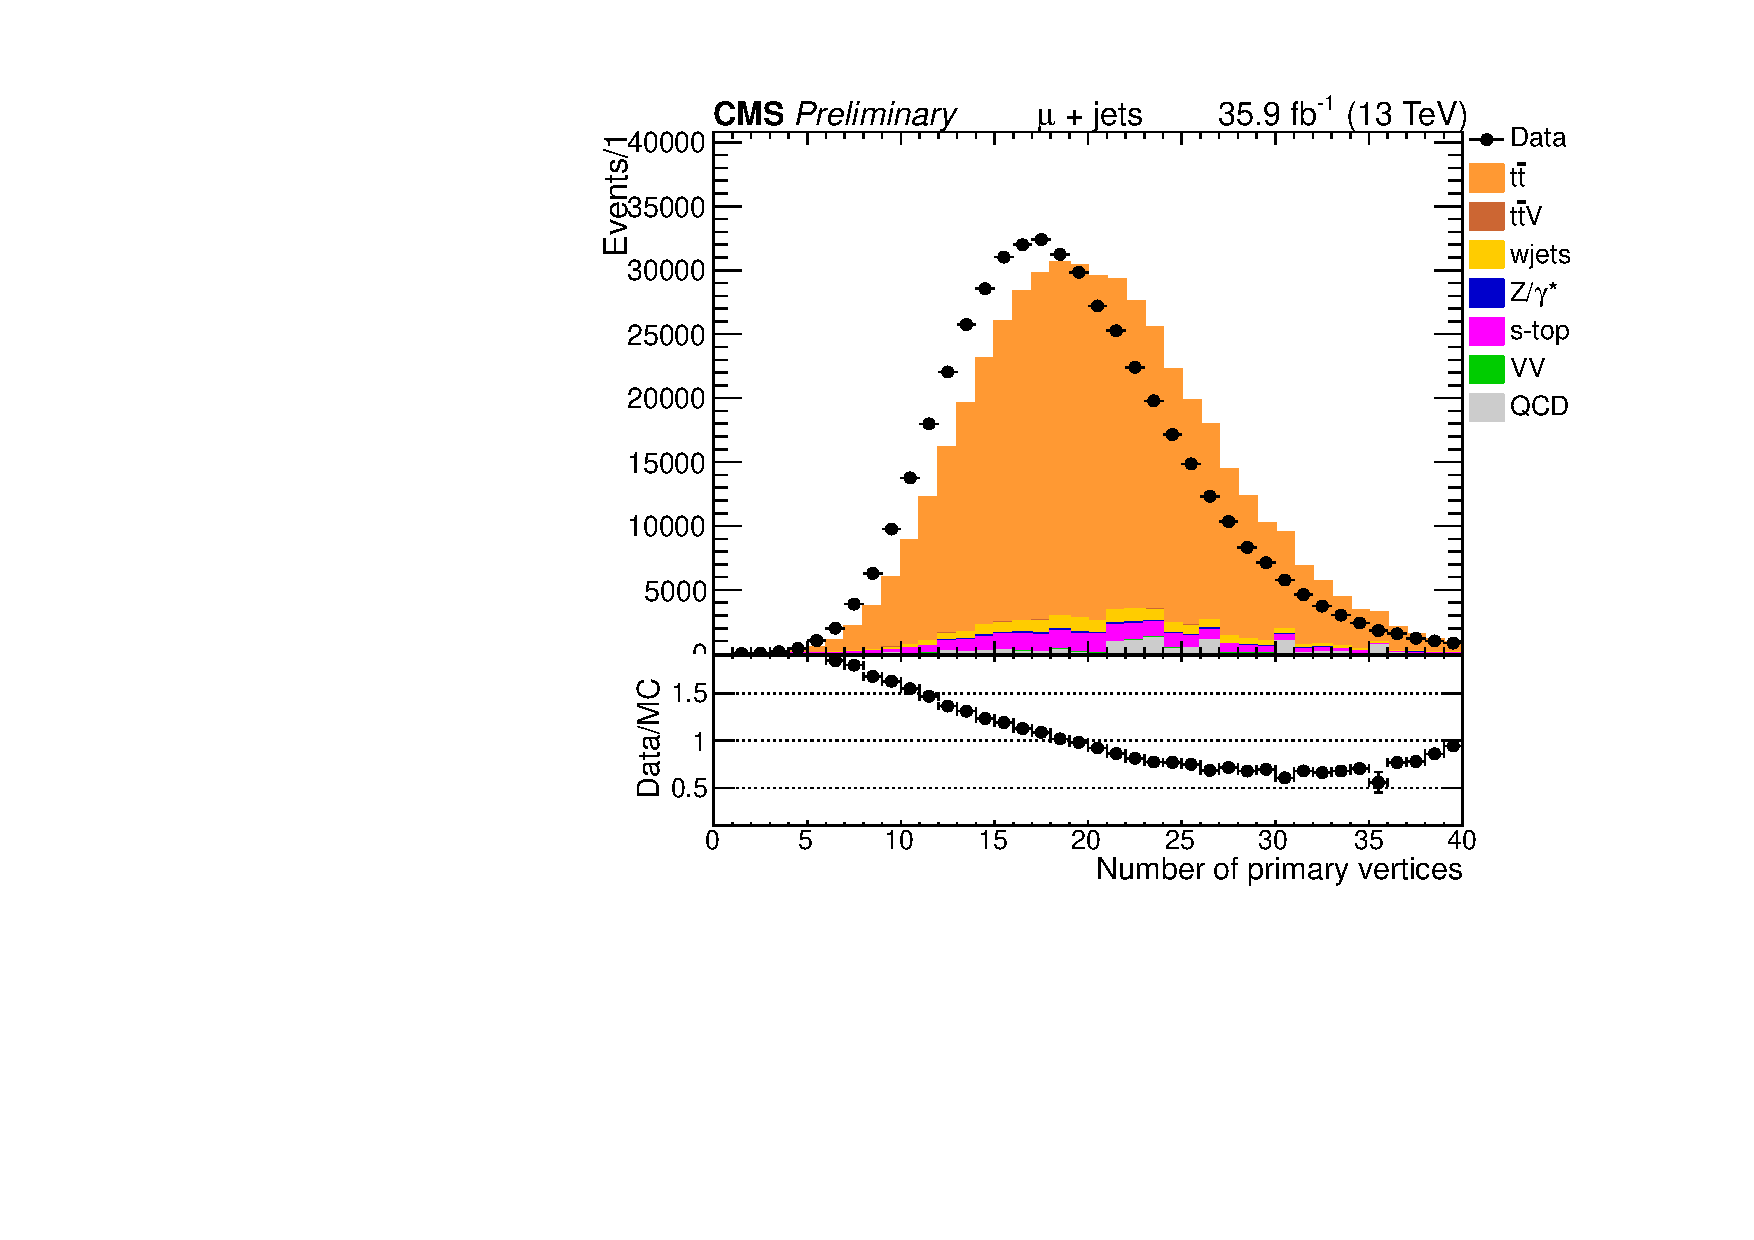
\includegraphics[width=0.45\textwidth]{fig/app4/muon/EvtInfo_NumVtx_w.pdf}
  \caption{Basic variables distributions in muon channel, from left to right, transverse momentum, $p_{T}$, and pseudorapidity, $\eta$, of leading b-jets, number of the selected b-jets and $m_{T}^{W}$, number of primary vertices without and with PU reweighting.}
  \label{Fig:DataMCMuon2}
  \end{figure}

\begin{figure}
  \centering
  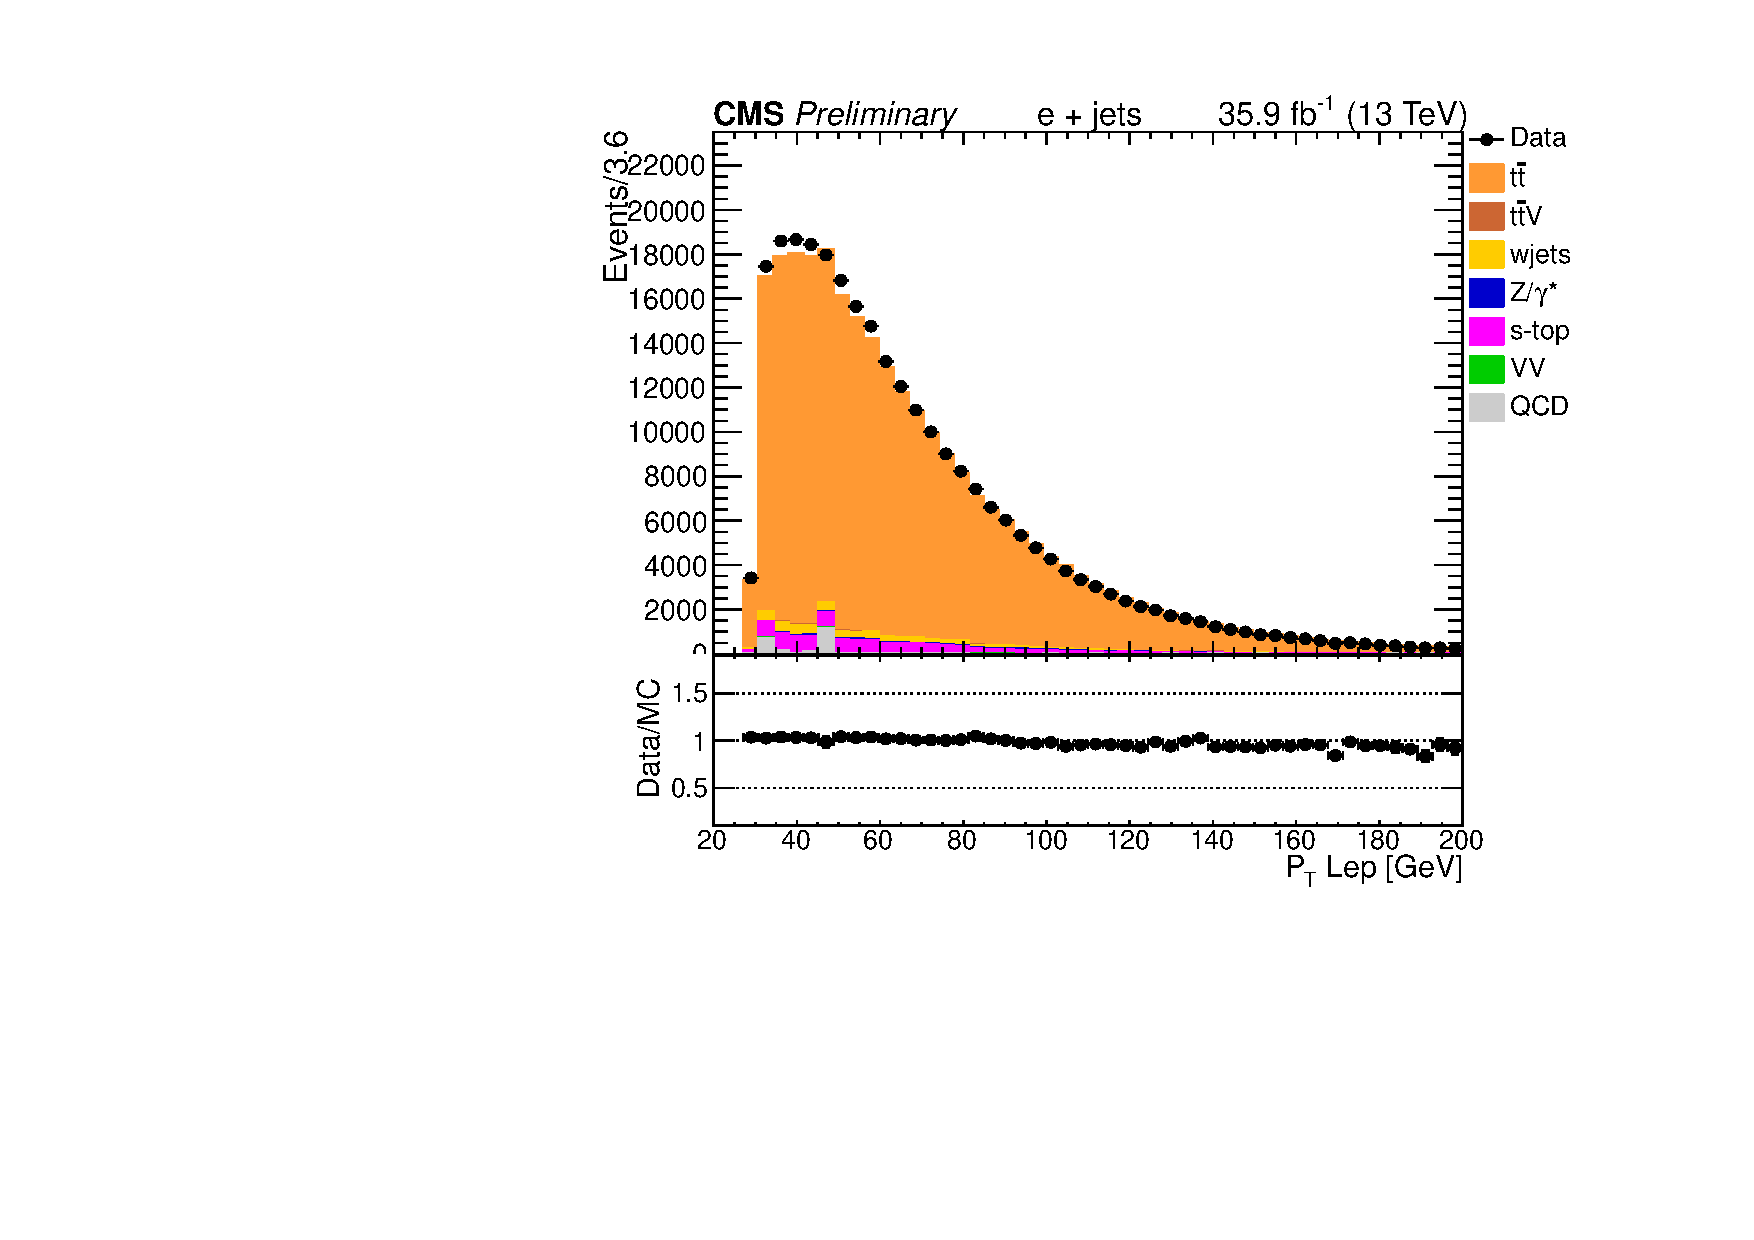
\includegraphics[width=0.45\textwidth]{fig/app4/ele/Pt_lep.pdf}
  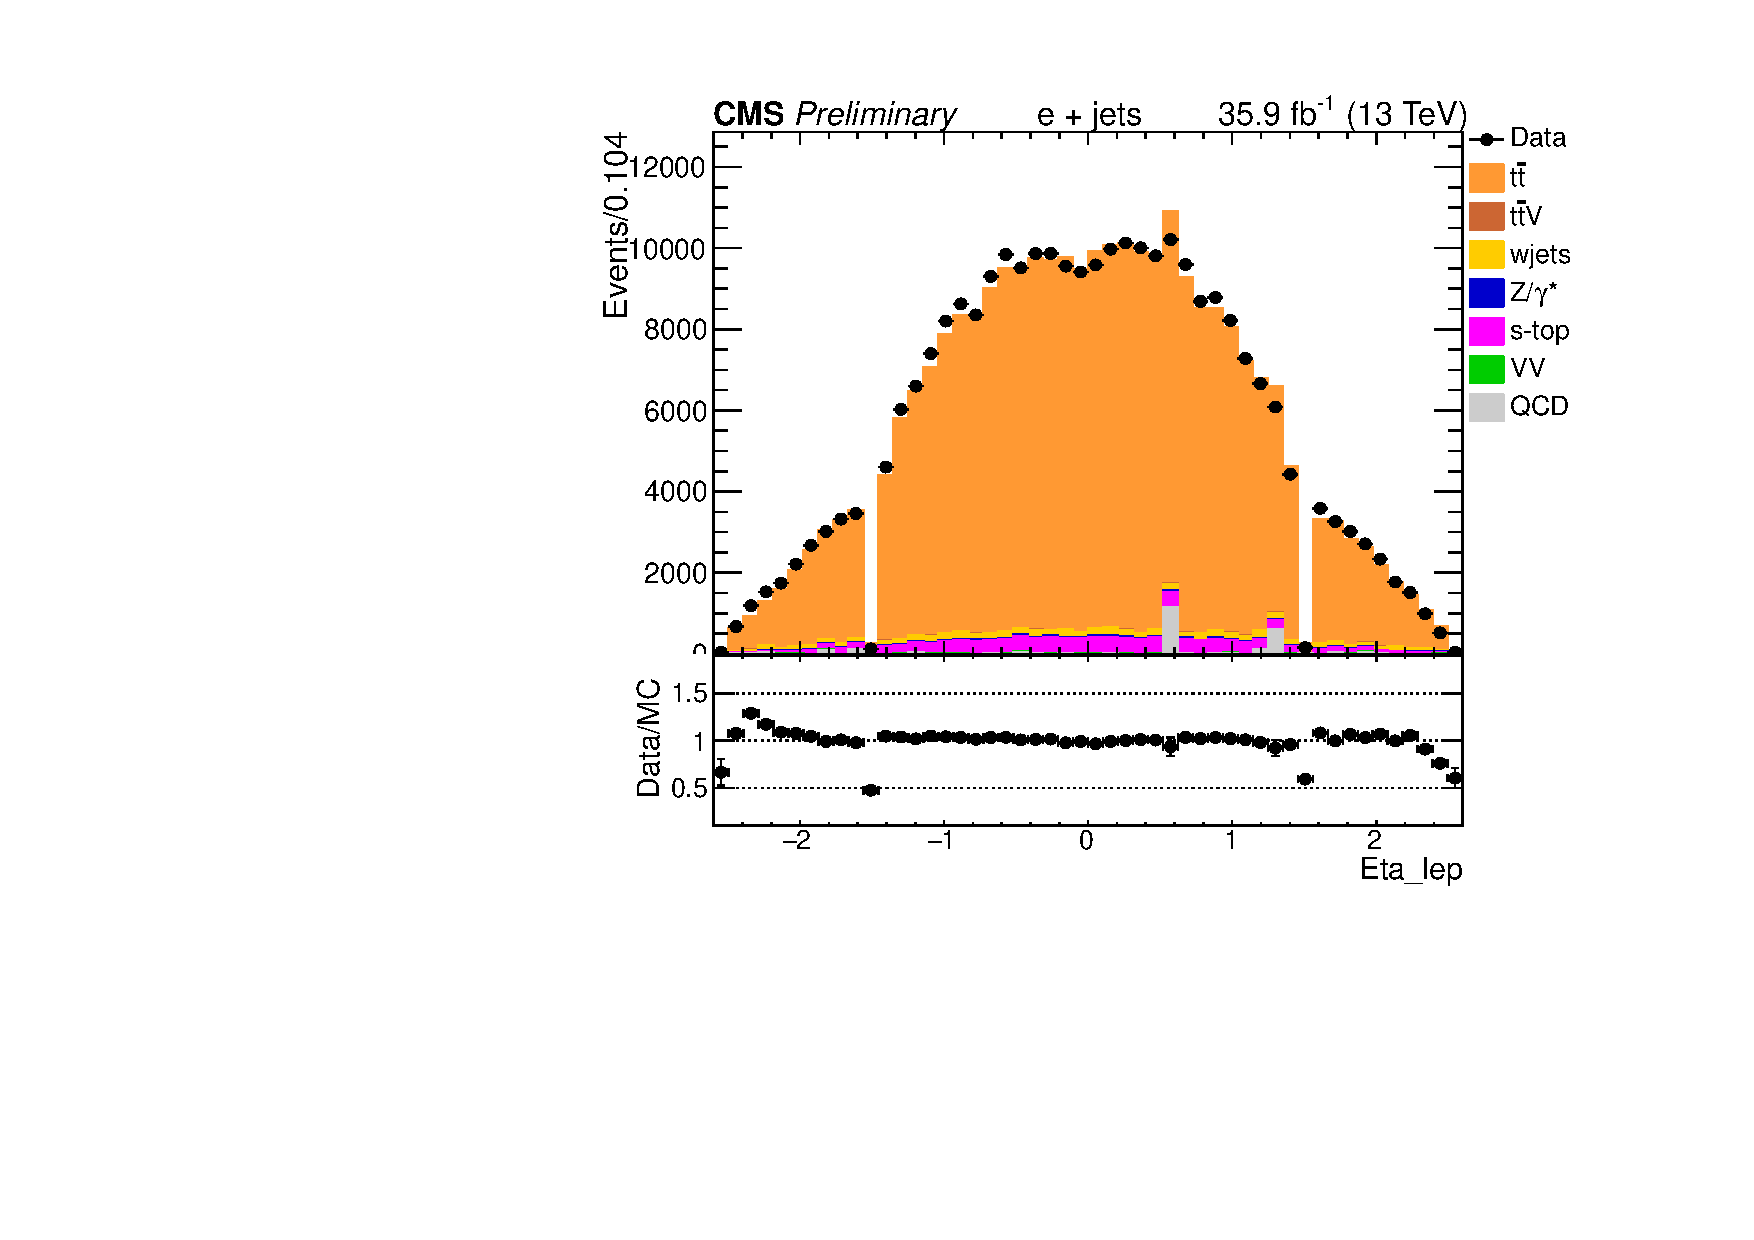
\includegraphics[width=0.45\textwidth]{fig/app4/ele/Eta_lep.pdf} \\
  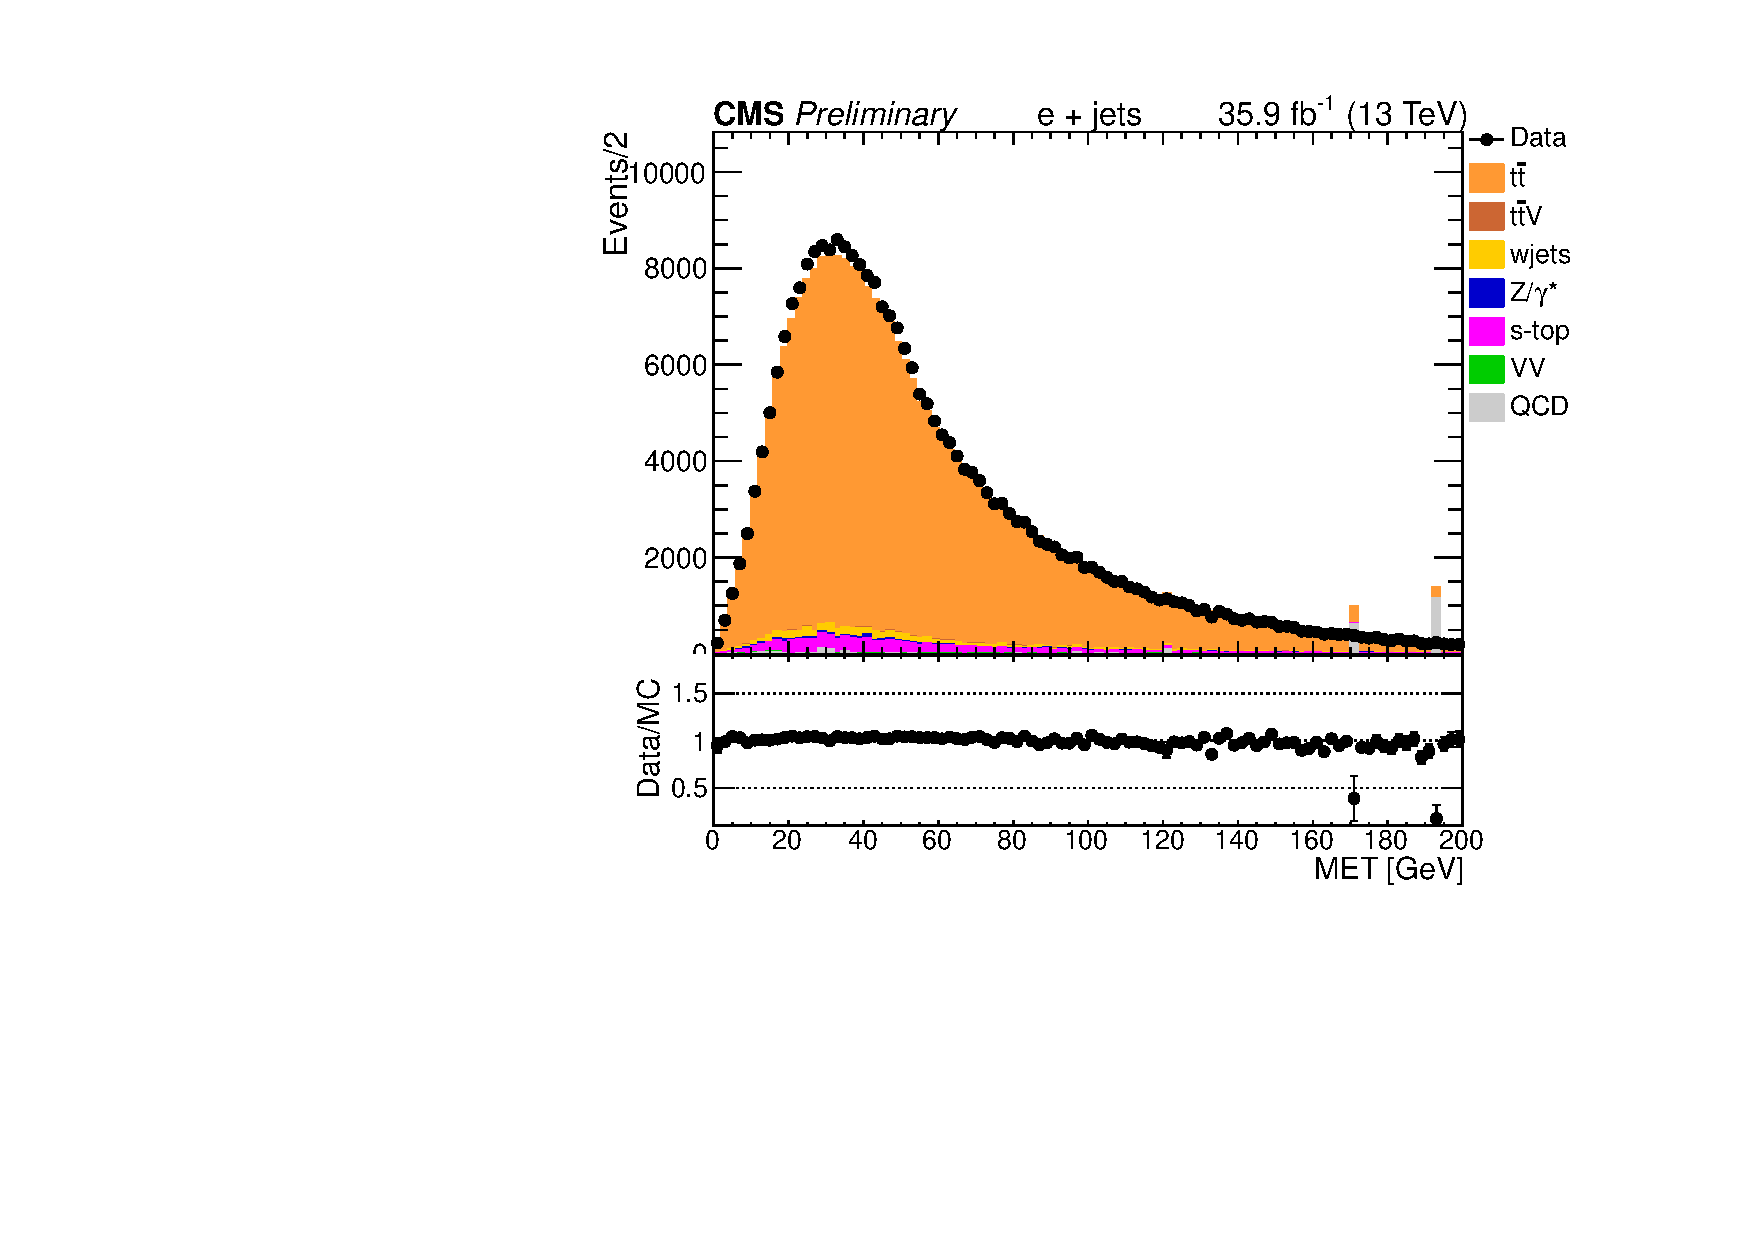
\includegraphics[width=0.45\textwidth]{fig/app4/ele/MET_E.pdf}
  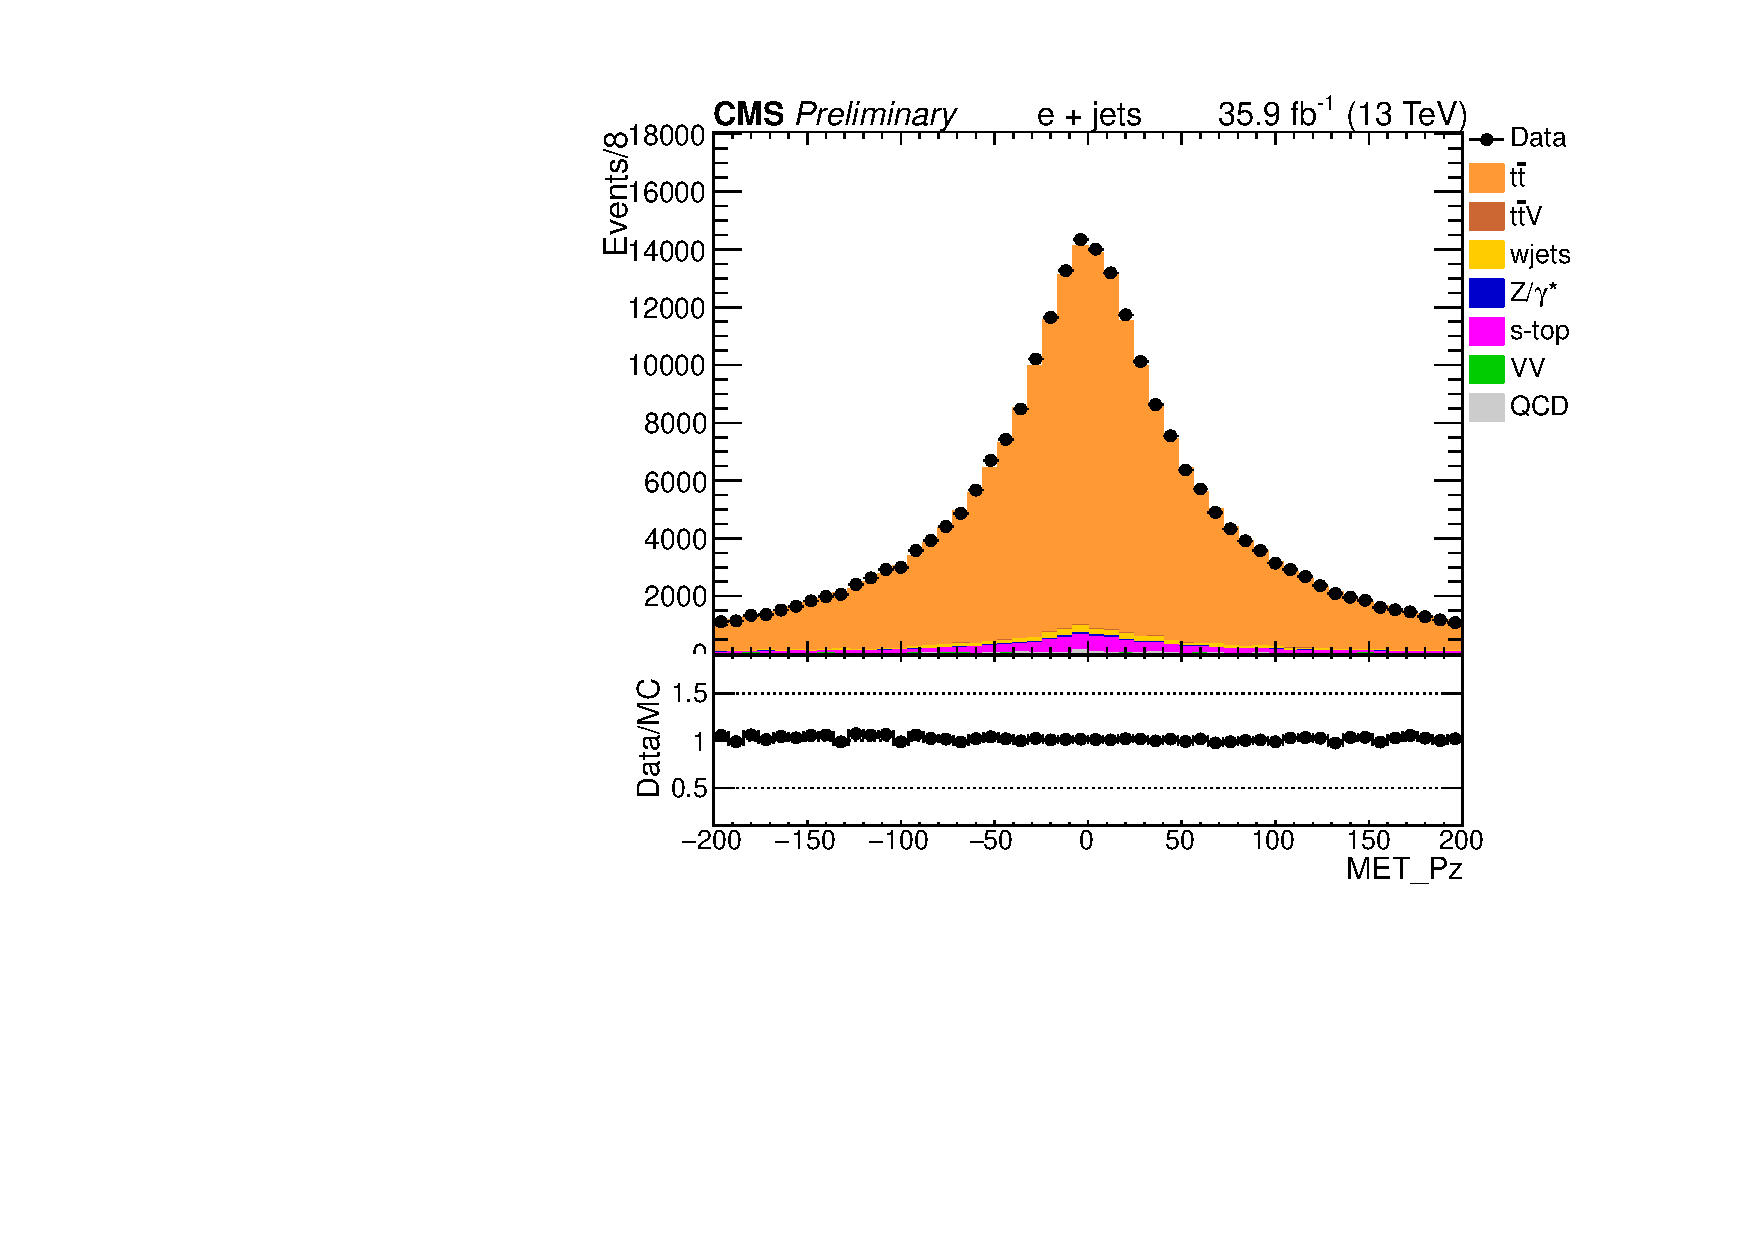
\includegraphics[width=0.45\textwidth]{fig/app4/ele/MET_Pz.pdf}
  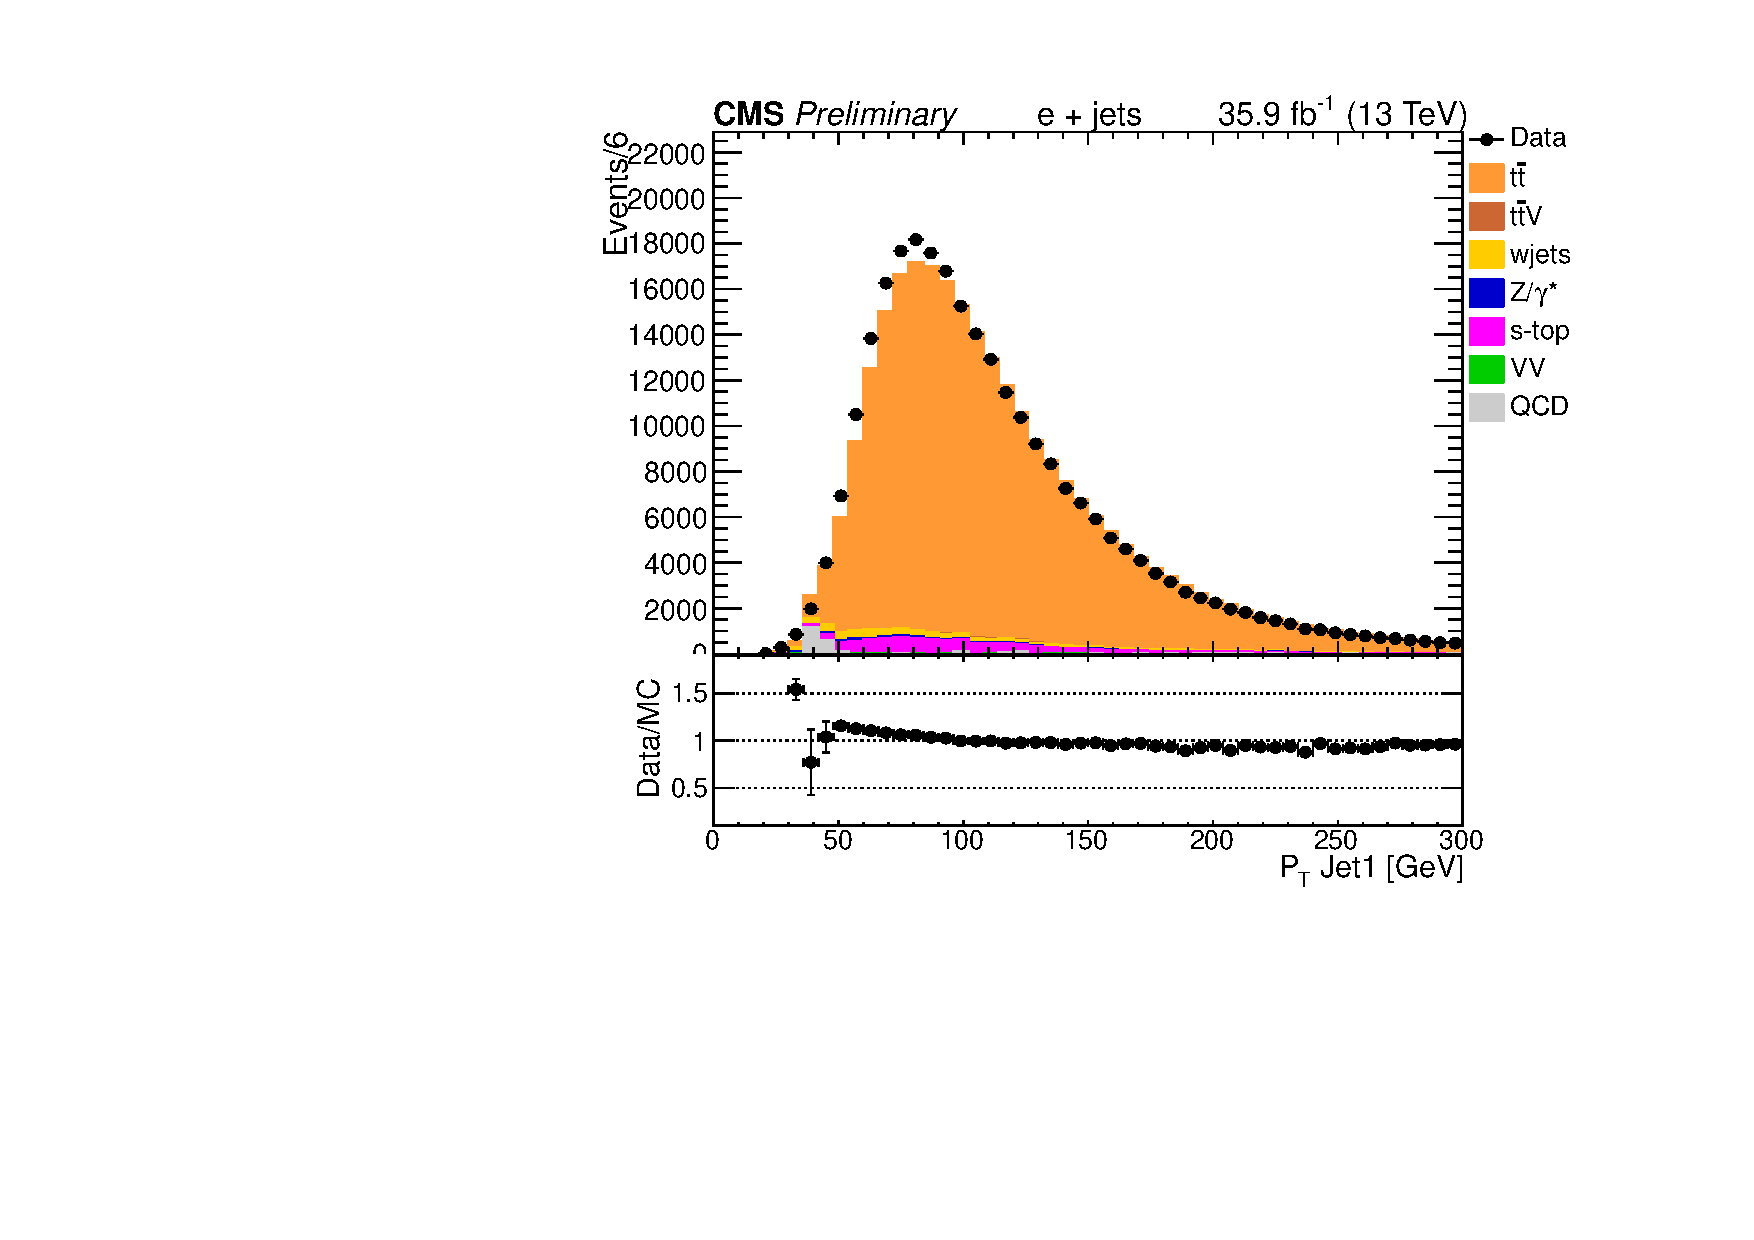
\includegraphics[width=0.45\textwidth]{fig/app4/ele/PtJet1.pdf}
  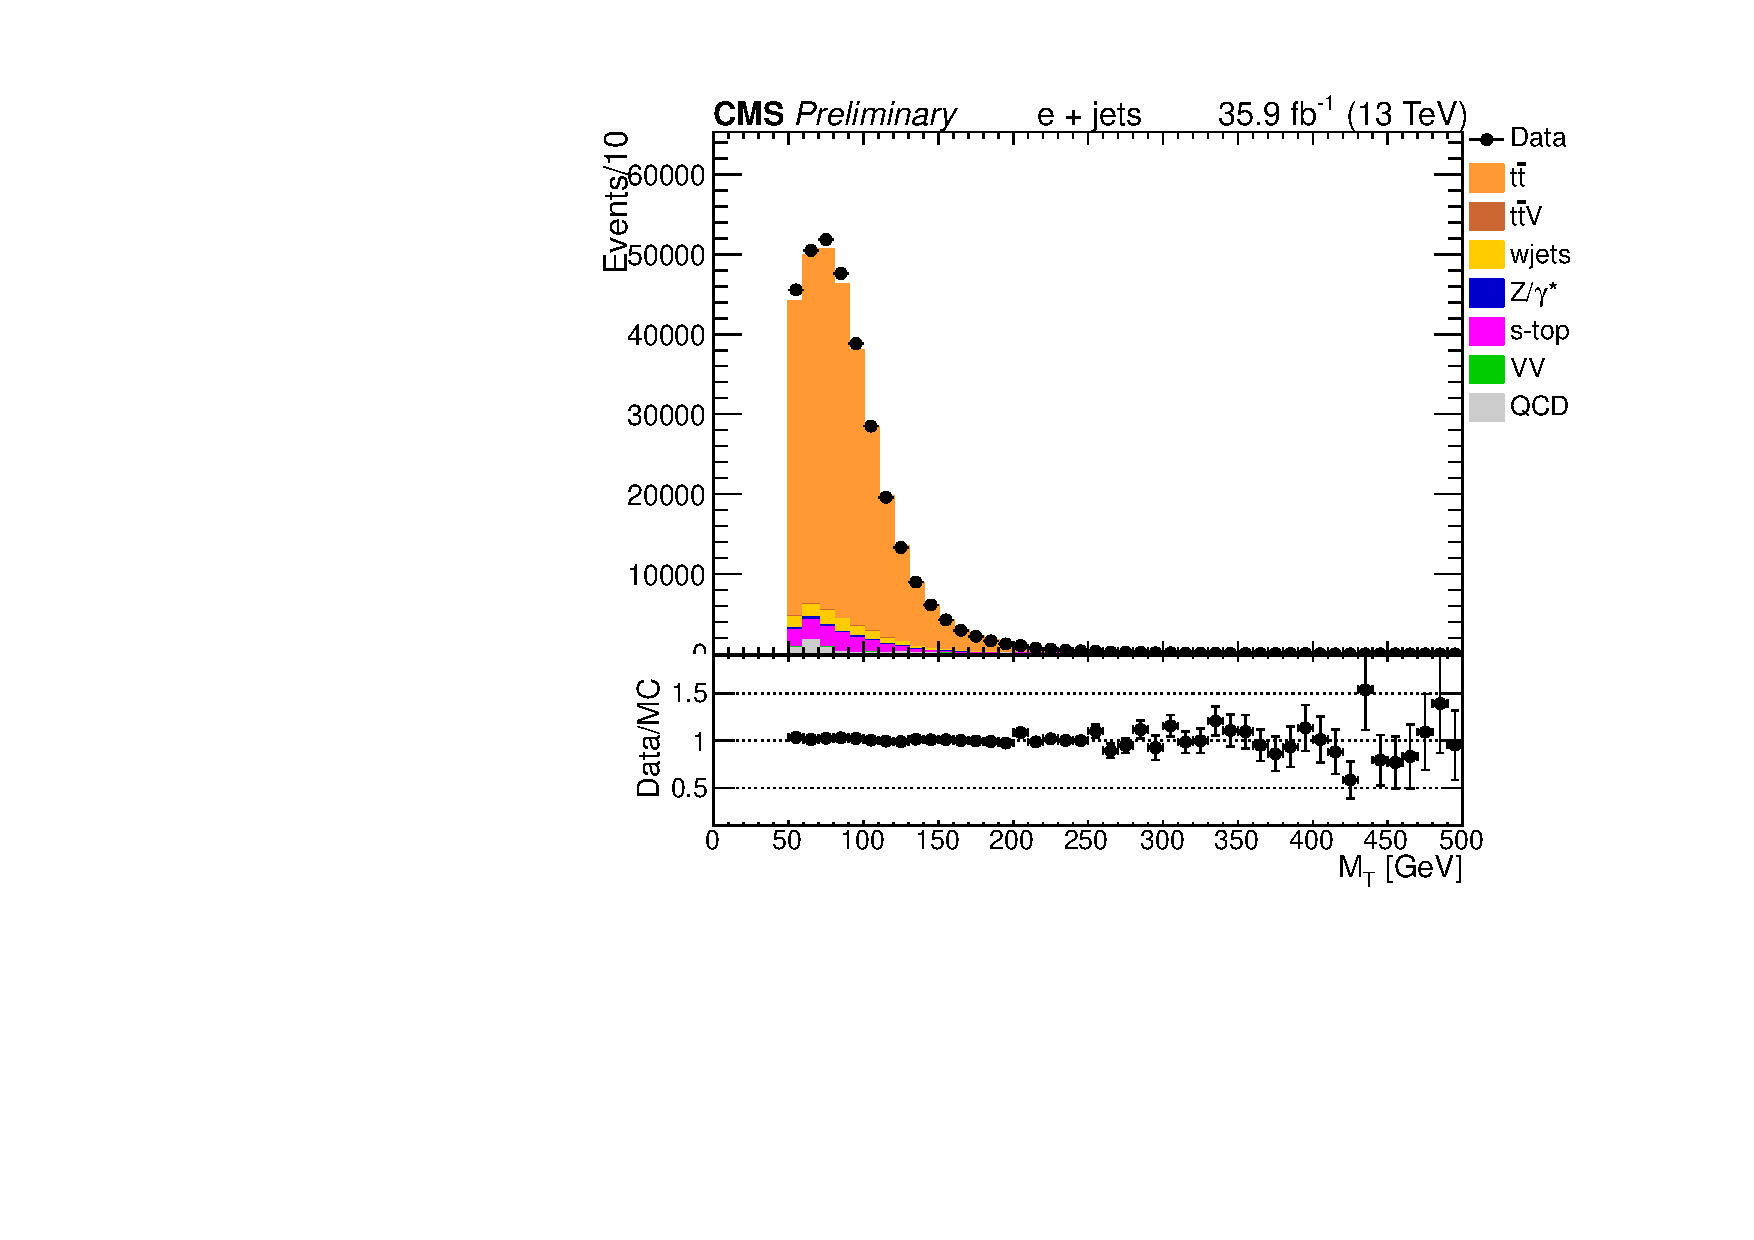
\includegraphics[width=0.45\textwidth]{fig/app4/ele/M_T_aft.pdf}
  \caption{Basic variables distributions in electron channel, from left to right, transverse momentum, $p_{T}$, and pseudorapidity, $\eta$, of electron, missing transverse energy, $p_{T}^{\text{miss}}$, and the corresponding reconstructed $p_{Z}$ of $p_{T}^{\text{miss}}$, leading $p_{T}$ of jets and $m_{T}^{W}$.}
  \label{Fig:DataMCLeptons}
  \end{figure}

\begin{figure}
  \centering
  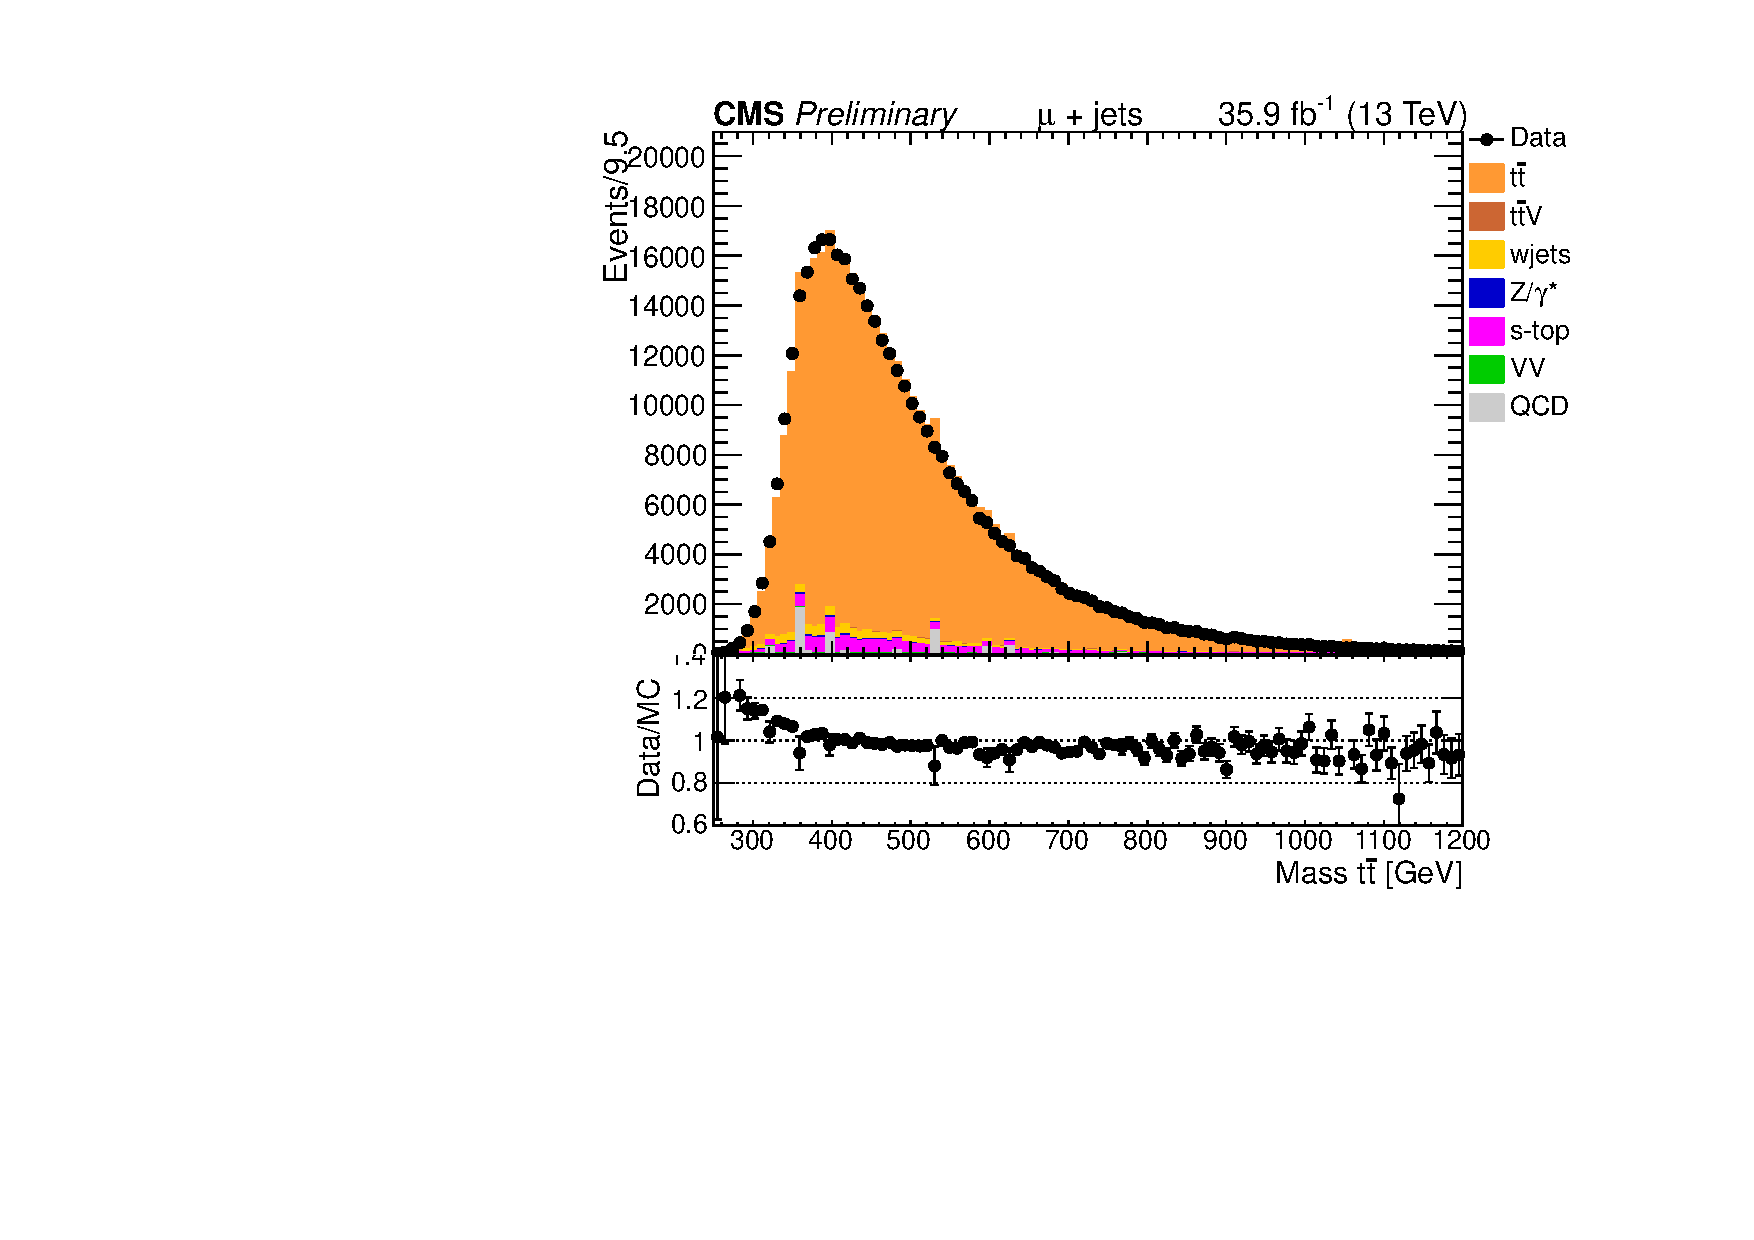
\includegraphics[width=0.45\textwidth]{fig/app4/muon/Mass_tt.pdf}
  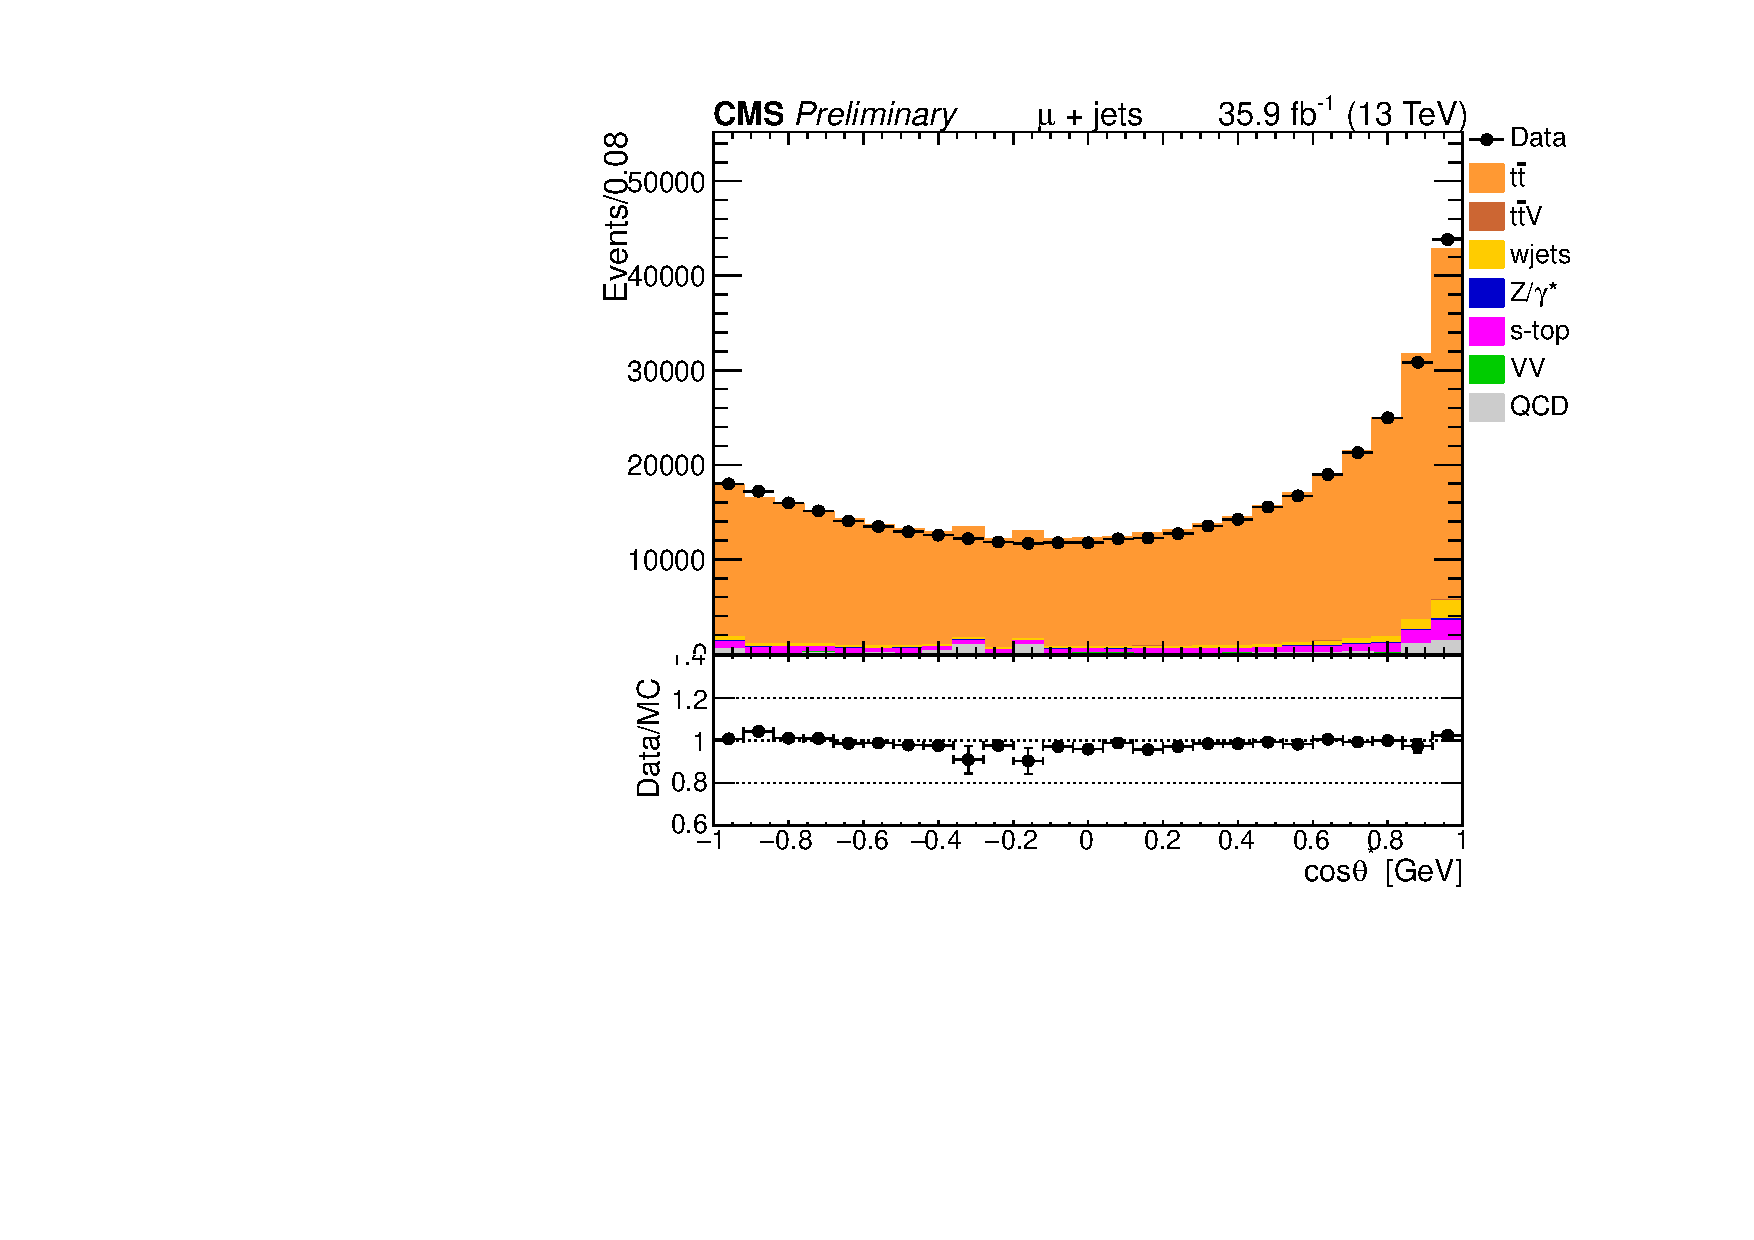
\includegraphics[width=0.45\textwidth]{fig/app4/muon/cos_theta.pdf} \\
  \caption{From left to right, mass of $t\bar t$ and $\cos\theta^*$ distributions in muon channel. Both of the variables used in the final statistical evaluation.}
  \label{Fig:DataMCMuon3}
  \end{figure}


\clearpage{\pagestyle{empty}\cleardoublepage}
